\section{Профиль и протокол}
\subsection{Цель и определения}
Цель --- оценить, когда уверенность замороженной модели соответствует ошибкам и где она перестаёт быть надёжной~\cite{teacher}. Accuracy и калибровка --- разные свойства. Для вероятностей $p=\operatorname{softmax}(z)$ уверенность $conf=\max_cp_c$, а калибровка требует $P(\hat Y=Y\mid conf=p)=p$. Использованы
\begin{equation}\begin{aligned}ECE=\sum_m\frac{|B_m|}{N}|acc(B_m)-conf(B_m)|,\quad NLL=-\frac1N\sum_i\log p_{y_i},\\ BS=\frac1N\sum_{i,c}(p_{ic}-1[y_i=c])^2.\end{aligned}\end{equation}
ECE зависит от интервалов и учитывает верхнюю вероятность; NLL и Brier используют весь вектор. Пустые интервалы не дают определённой accuracy и исключаются из суммы.

Температура $p^{(T)}=\operatorname{softmax}(z/T)$ при $T>0$ сохраняет argmax, но меняет вероятности. $\ln T$ минимизирует NLL только на val, с кандидатом T=1. Основные меры неопределённости, больше означает менее уверенно:
\begin{equation}U_{MSP}=1-\max_cp_c,\qquad H=-\sum_cp_c\ln p_c,\qquad U_{margin}=1-p_{(1)}+p_{(2)}.\end{equation}

\subsection{Данные, модели и искажения}
Профиль: CNN, основное искажение occlusion, PGD $\epsilon=2/255$. ECE: 15 интервалов равной ширины. Использованы сохранённые модели ЛР2, обученные на 2150 train-изображениях (доля 0.05) за 10 000 обновлений. Для CNN имеются три подлинных seed, поэтому test не делится на псевдонезависимые seed. ViT seed 1 служит вторым архитектурным ориентиром. Новые классификаторы не обучаются.
\begin{table}[H]\centering\small
\setlength{\tabcolsep}{4pt}
\caption{Использованные источники моделей ЛР2: доля train 0.05, 10 000 обновлений.}\label{tab:sources}
\begin{tabular}{ll ll}
\toprule
Модель & Seed & Архитектура & Источник \\
\midrule
CNN & 1 & ResNet-18 & R01 \\
CNN & 2 & ResNet-18 & R02 \\
CNN & 3 & ResNet-18 & R03 \\
VIT & 1 & ViT P4 D384 & R04 \\
\bottomrule
\end{tabular}
\end{table}


CIFAR-10: train 43 000, val 5000, cal 2000, test 10 000. Нормализация взята из train ЛР2 и применяется ровно один раз. T подбирается на val; cal не используется, поскольку дополнительное conformal prediction не выполняется. Все атаки и оценки используют общий полный test. Устройство --- RTX 3060 Laptop. Для semantic OOD использован полный test SVHN, 26 032 изображения, без смысловых меток цифр.

Реализованы пять локальных параметризованных искажений уровней 0--5. Gaussian noise: std 0,0.04,0.06,0.08,0.09,0.10; Gaussian blur: sigma 0,0.4,0.7,1.0,1.3,1.6; brightness: множители 1,1.15,1.30,1.45,1.60,1.75; contrast: 1,0.8,0.6,0.4,0.2,0.1; occlusion: доля площади 0,0.1,0.2,0.3,0.4,0.5. Это явные локальные приближения, а не сертифицированная реализация CIFAR-10-C. Они работают до нормализации в RGB [0,1], сохраняют форму и метку; уровень 0 тождественный.

\section{E1. Калибровка и температура}
\begin{table}[H]\centering\scriptsize
\setlength{\tabcolsep}{4pt}
\caption{E1: чистый test; ECE --- 15 интервалов равной ширины.}\label{tab:e1}
\begin{tabular}{lrrrrrrrl}
\toprule
Модель & $T$ & Accuracy & Conf. & ECE & NLL & Brier & Пусто & Ист. \\
\midrule
CNN & 1.00000 & 0.70740 & 0.92225 & 0.21485 & 1.64031 & 0.49371 & 3 & R05 \\
CNN & 2.95638 & 0.70740 & 0.72477 & 0.02842 & 0.90976 & 0.40894 & 2 & R05 \\
VIT & 1.00000 & 0.45020 & 0.91751 & 0.46731 & 4.06538 & 0.98785 & 4 & R06 \\
VIT & 4.27331 & 0.45020 & 0.49568 & 0.06678 & 1.67486 & 0.70922 & 5 & R06 \\
\bottomrule
\end{tabular}
\end{table}


Все 10 000 предсказанных классов каждой модели сохранены: разность accuracy равна нулю. CNN val NLL уменьшилась с 1.602649 до 0.890119. На test обе модели улучшили ECE, NLL и Brier. До масштабирования CNN одновременно точнее и лучше откалибрована; после него порядок сохраняется. Это наблюдаемая связь двух моделей, а не тождество точности и калибровки.
\begin{figure}[H]\centering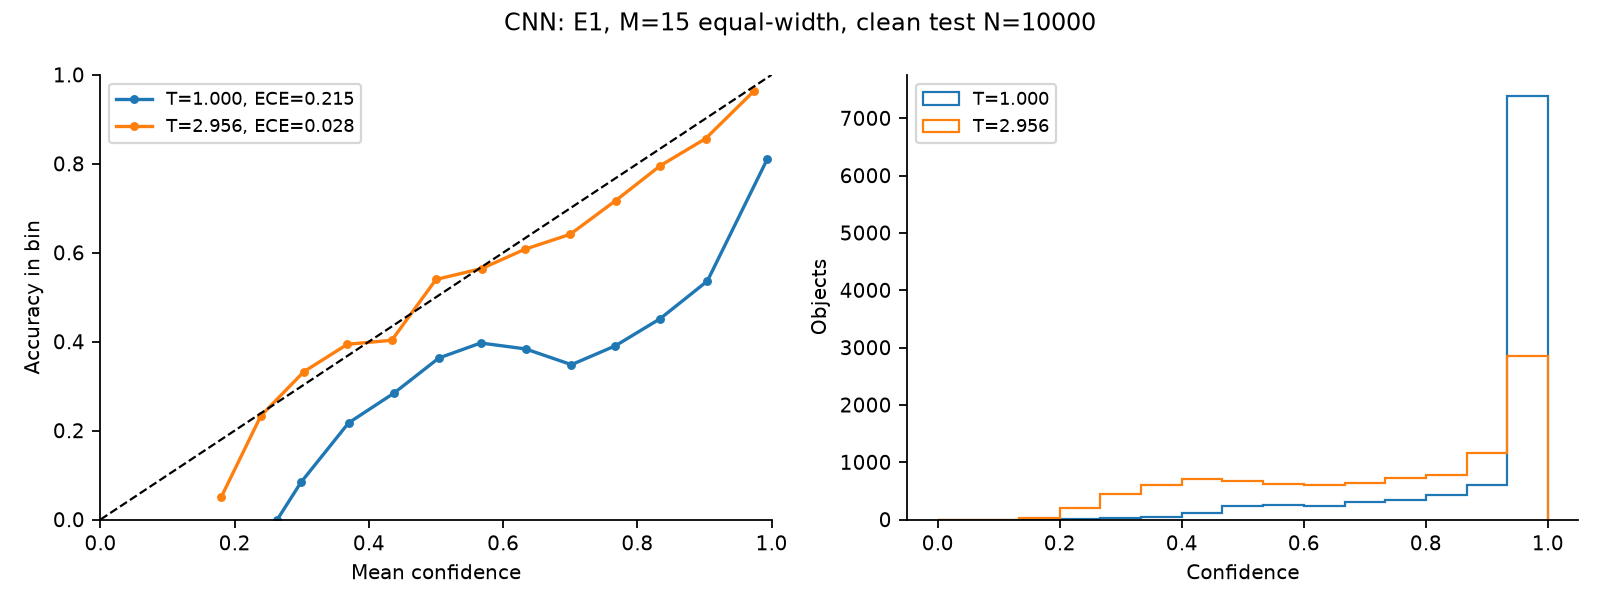
\includegraphics[width=\linewidth,height=.37\textheight,keepaspectratio]{figures/cnn.png}
\caption{CNN: reliability diagram и confidence до/после T*=2.956378; ECE 15 equal-width.}\label{fig:cnn}
\end{figure}

\begin{figure}[H]\centering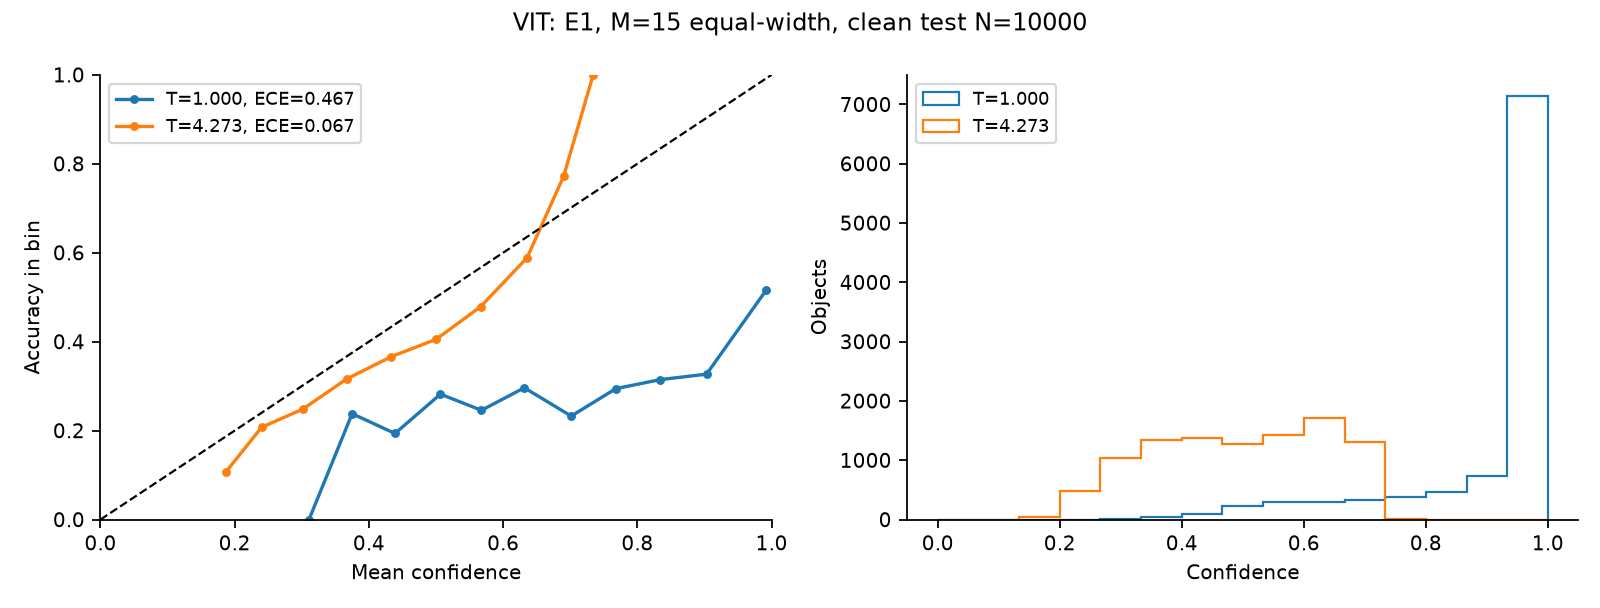
\includegraphics[width=\linewidth,height=.37\textheight,keepaspectratio]{figures/vit.png}
\caption{ViT: аналогичная оценка, T*=4.273313, ECE 15 equal-width.}\label{fig:vit}
\end{figure}

\begin{table}[H]\centering\footnotesize
\setlength{\tabcolsep}{4pt}
\caption{Граница E1: другие схемы ECE, те же предсказания.}\label{tab:binning}
\begin{tabular}{ll lrrr}
\toprule
Модель & M & Интервалы & $T$ & ECE & Пусто \\
\midrule
CNN & 5 & равной ширины & 1.0000 & 0.214846 & 1 \\
CNN & 50 & равной ширины & 1.0000 & 0.214846 & 13 \\
CNN & 15 & равное число & 1.0000 & 0.214846 & 0 \\
CNN & 5 & равной ширины & 2.9564 & 0.023358 & 0 \\
CNN & 50 & равной ширины & 2.9564 & 0.029443 & 8 \\
CNN & 15 & равное число & 2.9564 & 0.026857 & 0 \\
VIT & 5 & равной ширины & 1.0000 & 0.467313 & 1 \\
VIT & 50 & равной ширины & 1.0000 & 0.467313 & 13 \\
VIT & 15 & равное число & 1.0000 & 0.467313 & 0 \\
VIT & 5 & равной ширины & 4.2733 & 0.050628 & 1 \\
VIT & 50 & равной ширины & 4.2733 & 0.070663 & 20 \\
VIT & 15 & равное число & 4.2733 & 0.067447 & 0 \\
\bottomrule
\end{tabular}
\end{table}


\begin{figure}[H]\centering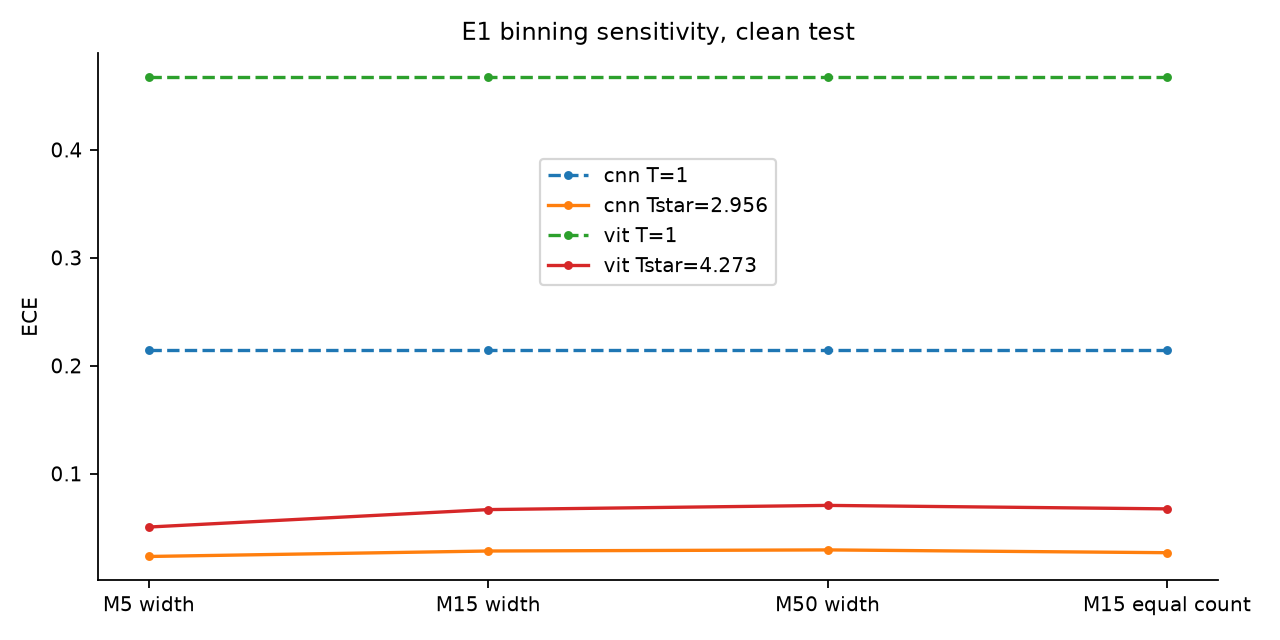
\includegraphics[width=\linewidth,height=.32\textheight,keepaspectratio]{figures/bins.png}
\caption{ECE при изменении схемы интервалов для обеих моделей.}\label{fig:bins}
\end{figure}

Вывод о снижении ECE сохраняется при 5 и 50 интервалах равной ширины и при 15 интервалах с равным числом объектов. Значения при разных схемах сравниваются только внутри одной схемы. Они не доказывают идеальную калибровку каждого отдельного класса или объекта.

\section{E2. Перенос температуры на искажённые данные}
CNN seed 1 исследована при всех пяти типах и шести уровнях; веса и T* с чистой val фиксированы. В таблице значения после масштабирования помечены индексом T. Accuracy одинакова при обеих температурах.
\begin{table}[H]\centering\scriptsize
\setlength{\tabcolsep}{4pt}
\caption{E2: CNN seed 1, общий test; индексы 1 и T обозначают температуры 1 и $T^*$.}\label{tab:grid}
\begin{tabular}{lrrrrrrrr}
\toprule
Искажение & $\ell$ & Acc. & $Conf_1$ & $Conf_T$ & $ECE_1$ & $ECE_T$ & $NLL_1$ & $NLL_T$ \\
\midrule
Шум & 0 & 0.7074 & 0.9222 & 0.7248 & 0.2148 & 0.0284 & 1.6403 & 0.9098 \\
Шум & 1 & 0.6834 & 0.9140 & 0.7082 & 0.2306 & 0.0299 & 1.7810 & 0.9800 \\
Шум & 2 & 0.6452 & 0.9074 & 0.6890 & 0.2622 & 0.0444 & 2.0642 & 1.1025 \\
Шум & 3 & 0.5926 & 0.8974 & 0.6661 & 0.3048 & 0.0746 & 2.4767 & 1.2743 \\
Шум & 4 & 0.5597 & 0.8938 & 0.6561 & 0.3341 & 0.0964 & 2.7234 & 1.3726 \\
Шум & 5 & 0.5284 & 0.8899 & 0.6470 & 0.3615 & 0.1188 & 2.9892 & 1.4759 \\
Размытие & 0 & 0.7074 & 0.9222 & 0.7248 & 0.2148 & 0.0284 & 1.6403 & 0.9098 \\
Размытие & 1 & 0.7004 & 0.9192 & 0.7197 & 0.2188 & 0.0265 & 1.6694 & 0.9256 \\
Размытие & 2 & 0.5841 & 0.8984 & 0.6679 & 0.3151 & 0.0840 & 2.4963 & 1.2734 \\
Размытие & 3 & 0.4369 & 0.8781 & 0.6172 & 0.4412 & 0.1816 & 3.8016 & 1.7857 \\
Размытие & 4 & 0.3211 & 0.8703 & 0.5938 & 0.5492 & 0.2728 & 4.9671 & 2.2141 \\
Размытие & 5 & 0.2668 & 0.8637 & 0.5781 & 0.5969 & 0.3113 & 5.5802 & 2.4465 \\
Яркость & 0 & 0.7074 & 0.9222 & 0.7248 & 0.2148 & 0.0284 & 1.6403 & 0.9098 \\
Яркость & 1 & 0.6942 & 0.9193 & 0.7183 & 0.2251 & 0.0290 & 1.7271 & 0.9480 \\
Яркость & 2 & 0.6738 & 0.9136 & 0.7030 & 0.2398 & 0.0385 & 1.9023 & 1.0289 \\
Яркость & 3 & 0.6322 & 0.9059 & 0.6840 & 0.2741 & 0.0519 & 2.1684 & 1.1456 \\
Яркость & 4 & 0.5913 & 0.8973 & 0.6650 & 0.3061 & 0.0739 & 2.4919 & 1.2815 \\
Яркость & 5 & 0.5507 & 0.8909 & 0.6481 & 0.3402 & 0.0974 & 2.8553 & 1.4281 \\
Контраст & 0 & 0.7074 & 0.9222 & 0.7248 & 0.2148 & 0.0284 & 1.6403 & 0.9098 \\
Контраст & 1 & 0.6946 & 0.9162 & 0.7123 & 0.2218 & 0.0286 & 1.6995 & 0.9460 \\
Контраст & 2 & 0.6348 & 0.8984 & 0.6691 & 0.2639 & 0.0364 & 2.0089 & 1.1116 \\
Контраст & 3 & 0.4779 & 0.8648 & 0.5909 & 0.3871 & 0.1130 & 3.0512 & 1.5797 \\
Контраст & 4 & 0.2040 & 0.8468 & 0.5483 & 0.6428 & 0.3443 & 6.4212 & 2.7752 \\
Контраст & 5 & 0.1524 & 0.8479 & 0.5297 & 0.6955 & 0.3773 & 7.7569 & 3.2450 \\
Закрытие & 0 & 0.7074 & 0.9222 & 0.7248 & 0.2148 & 0.0284 & 1.6403 & 0.9098 \\
Закрытие & 1 & 0.6301 & 0.8940 & 0.6567 & 0.2639 & 0.0332 & 2.0049 & 1.1311 \\
Закрытие & 2 & 0.5343 & 0.8647 & 0.5873 & 0.3304 & 0.0530 & 2.5039 & 1.4081 \\
Закрытие & 3 & 0.3911 & 0.8200 & 0.5066 & 0.4289 & 0.1155 & 3.3605 & 1.8285 \\
Закрытие & 4 & 0.3230 & 0.7954 & 0.4676 & 0.4724 & 0.1446 & 3.7742 & 2.0323 \\
Закрытие & 5 & 0.2447 & 0.7528 & 0.4133 & 0.5081 & 0.1686 & 4.3104 & 2.3025 \\
\bottomrule
\end{tabular}
\end{table}


\begin{figure}[H]\centering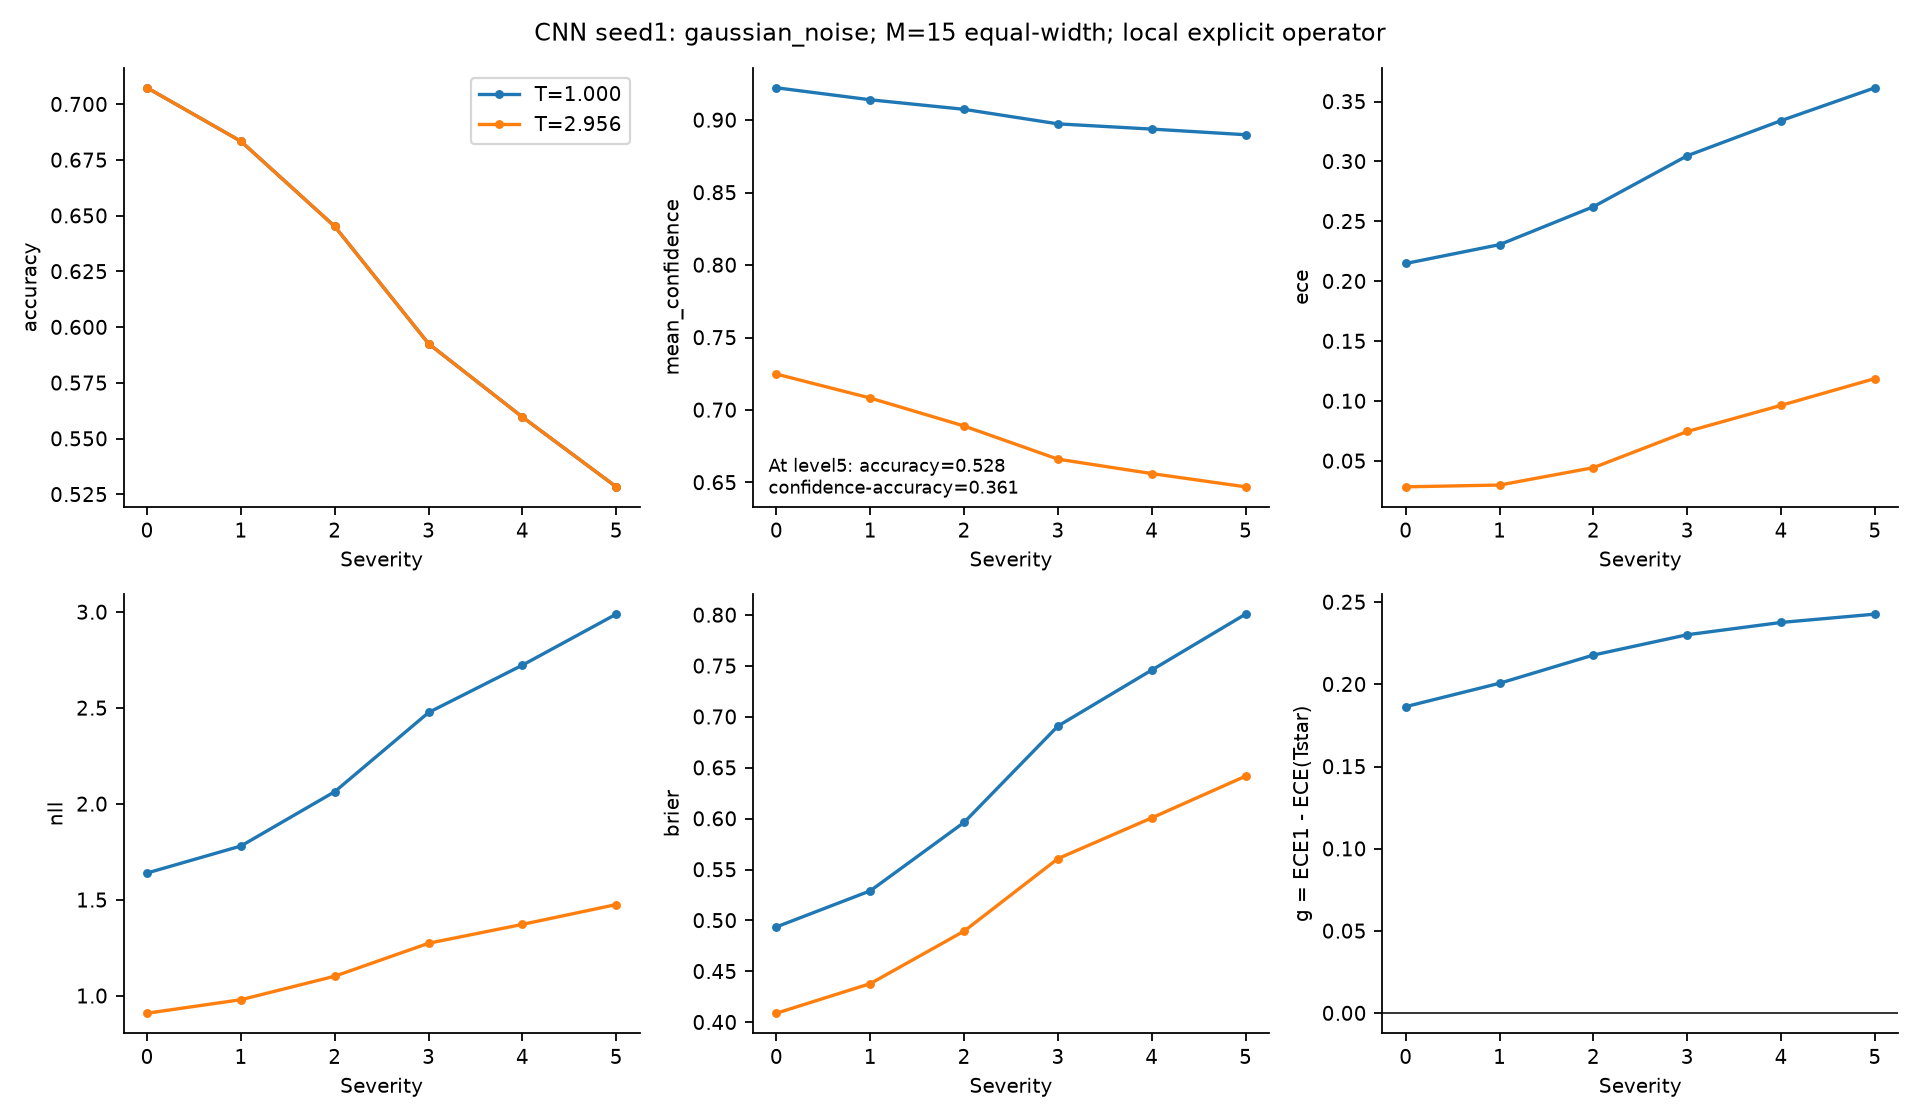
\includegraphics[width=\linewidth,height=.34\textheight,keepaspectratio]{figures/gaussian_noise.png}
\caption{E2: Шум, CNN seed 1; ECE 15 equal-width, T=1 и T*=2.956378.}\label{fig:gaussian_noise}
\end{figure}

\begin{figure}[H]\centering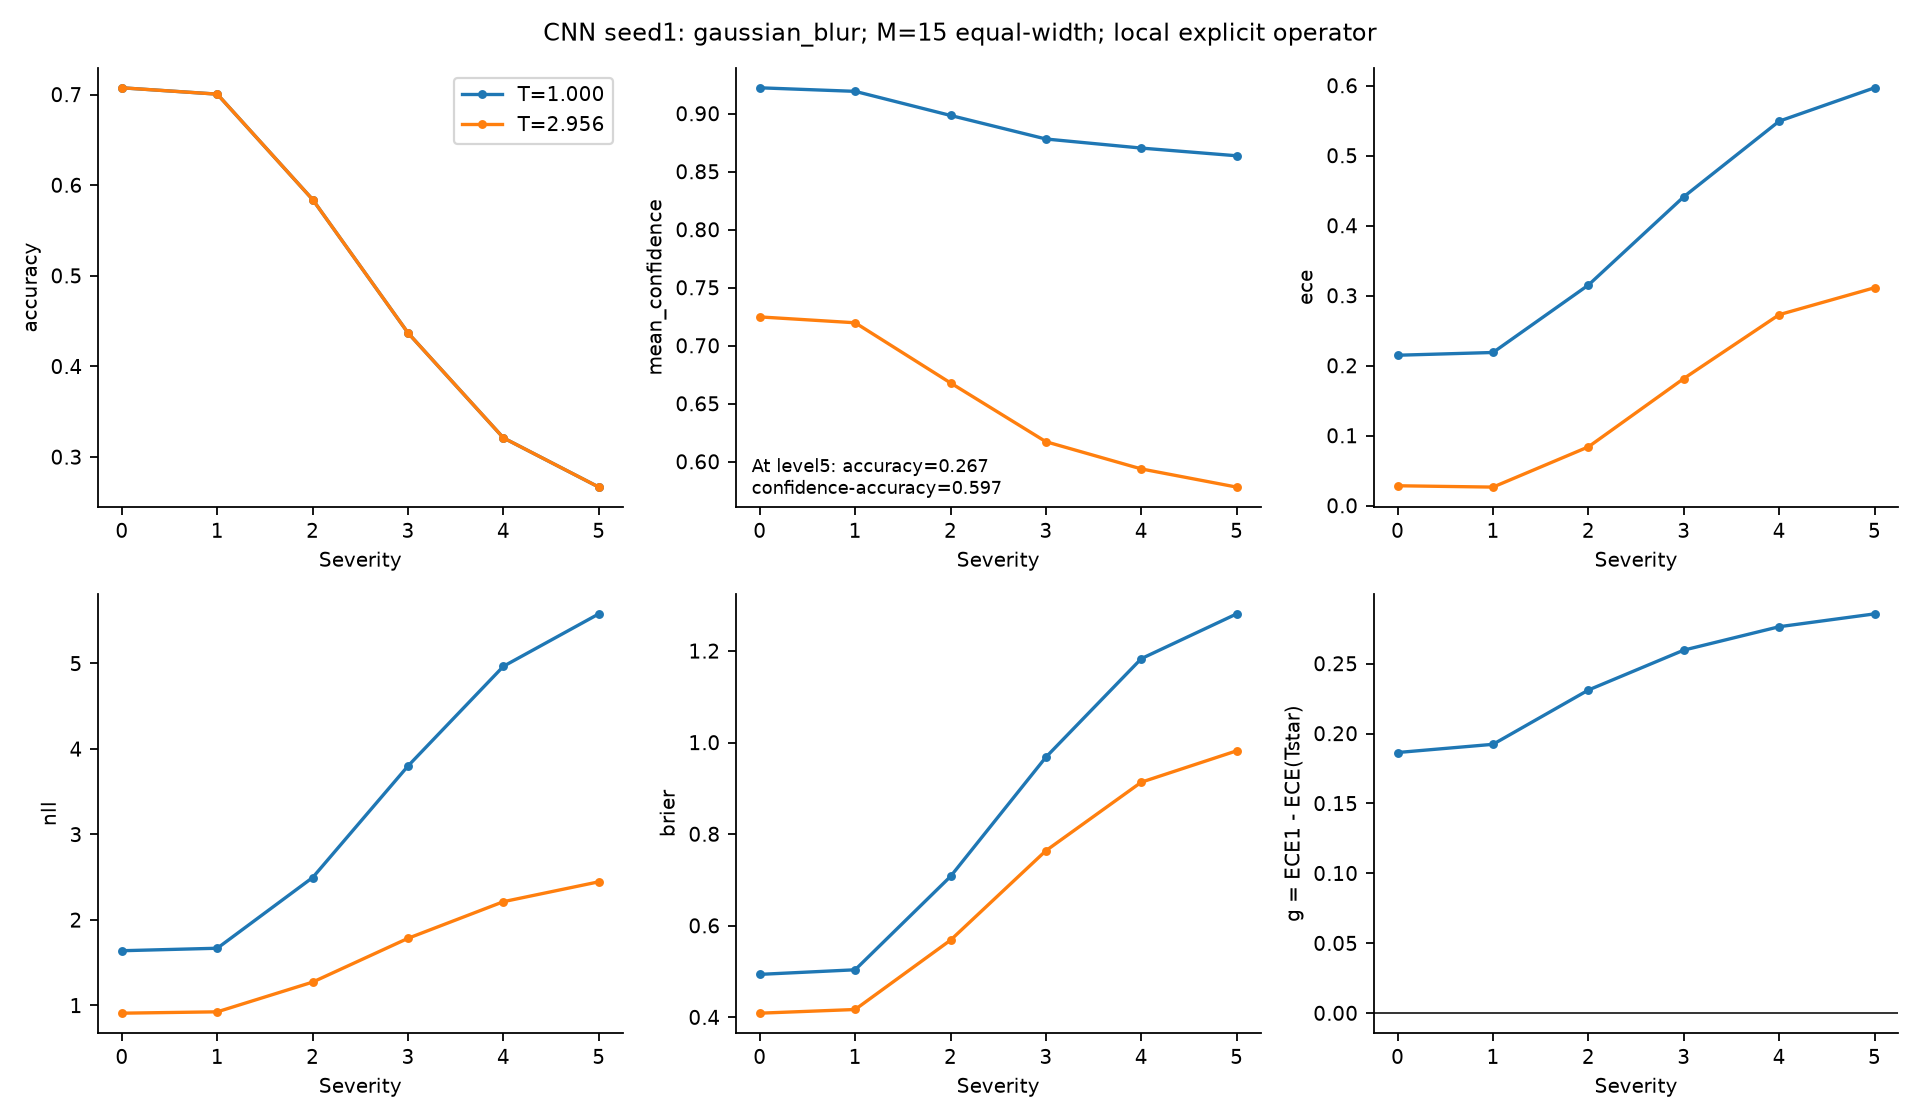
\includegraphics[width=\linewidth,height=.34\textheight,keepaspectratio]{figures/gaussian_blur.png}
\caption{E2: Размытие, CNN seed 1; ECE 15 equal-width, T=1 и T*=2.956378.}\label{fig:gaussian_blur}
\end{figure}

\begin{figure}[H]\centering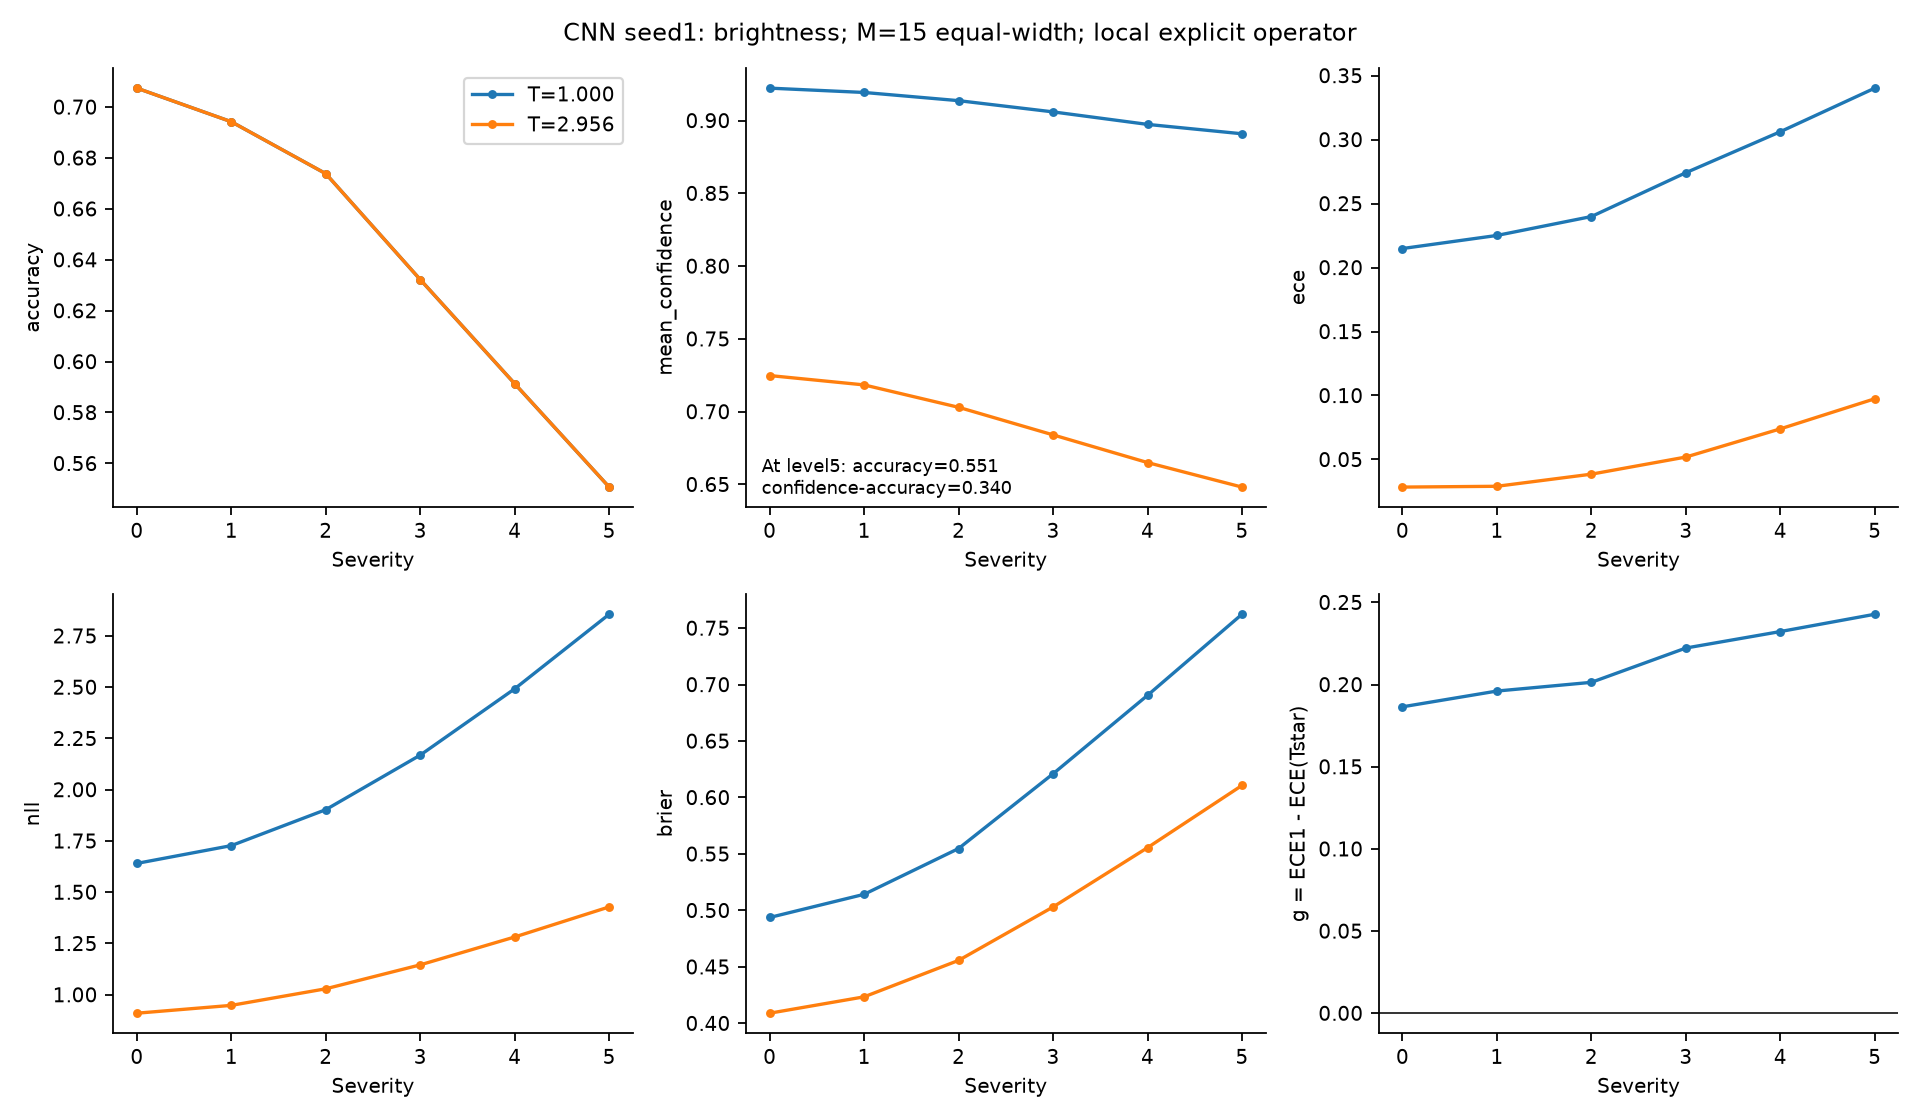
\includegraphics[width=\linewidth,height=.34\textheight,keepaspectratio]{figures/brightness.png}
\caption{E2: Яркость, CNN seed 1; ECE 15 equal-width, T=1 и T*=2.956378.}\label{fig:brightness}
\end{figure}

\begin{figure}[H]\centering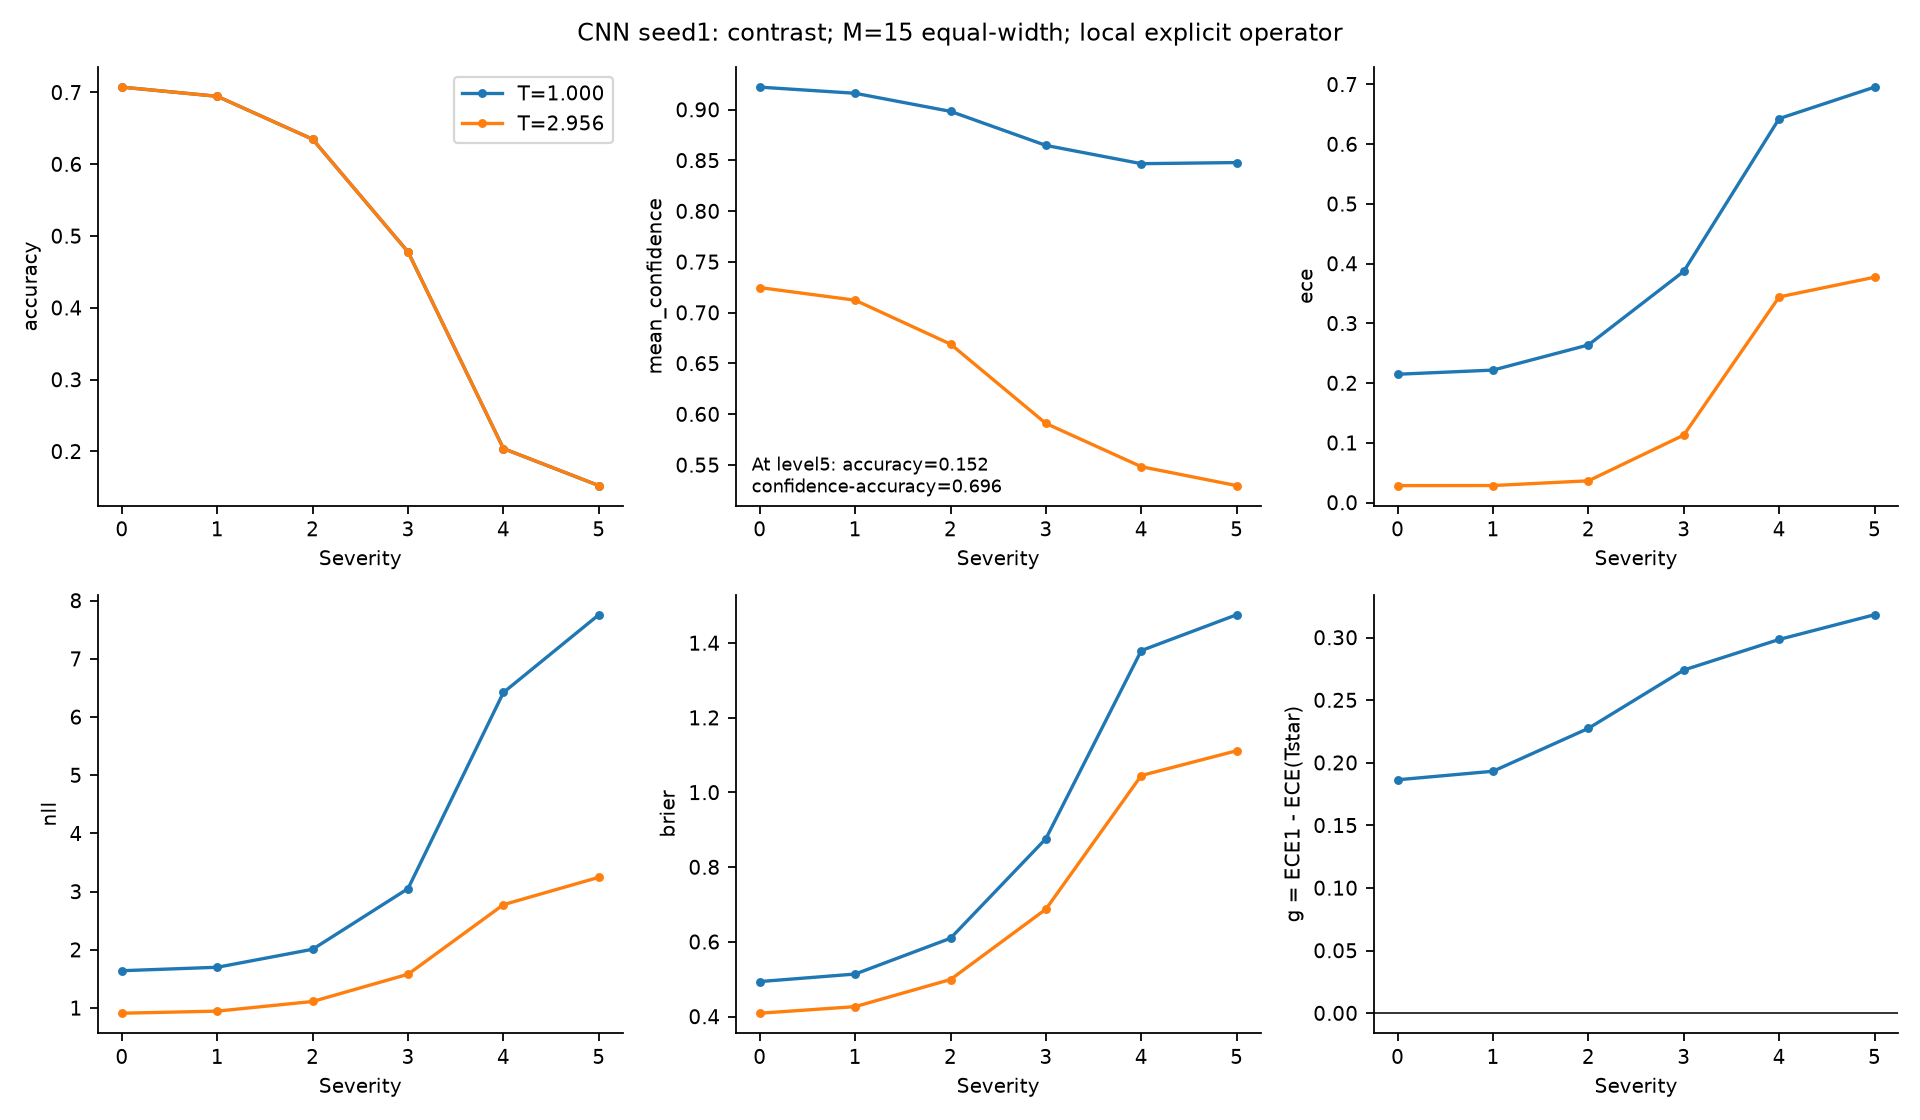
\includegraphics[width=\linewidth,height=.34\textheight,keepaspectratio]{figures/contrast.png}
\caption{E2: Контраст, CNN seed 1; ECE 15 equal-width, T=1 и T*=2.956378.}\label{fig:contrast}
\end{figure}

\begin{figure}[H]\centering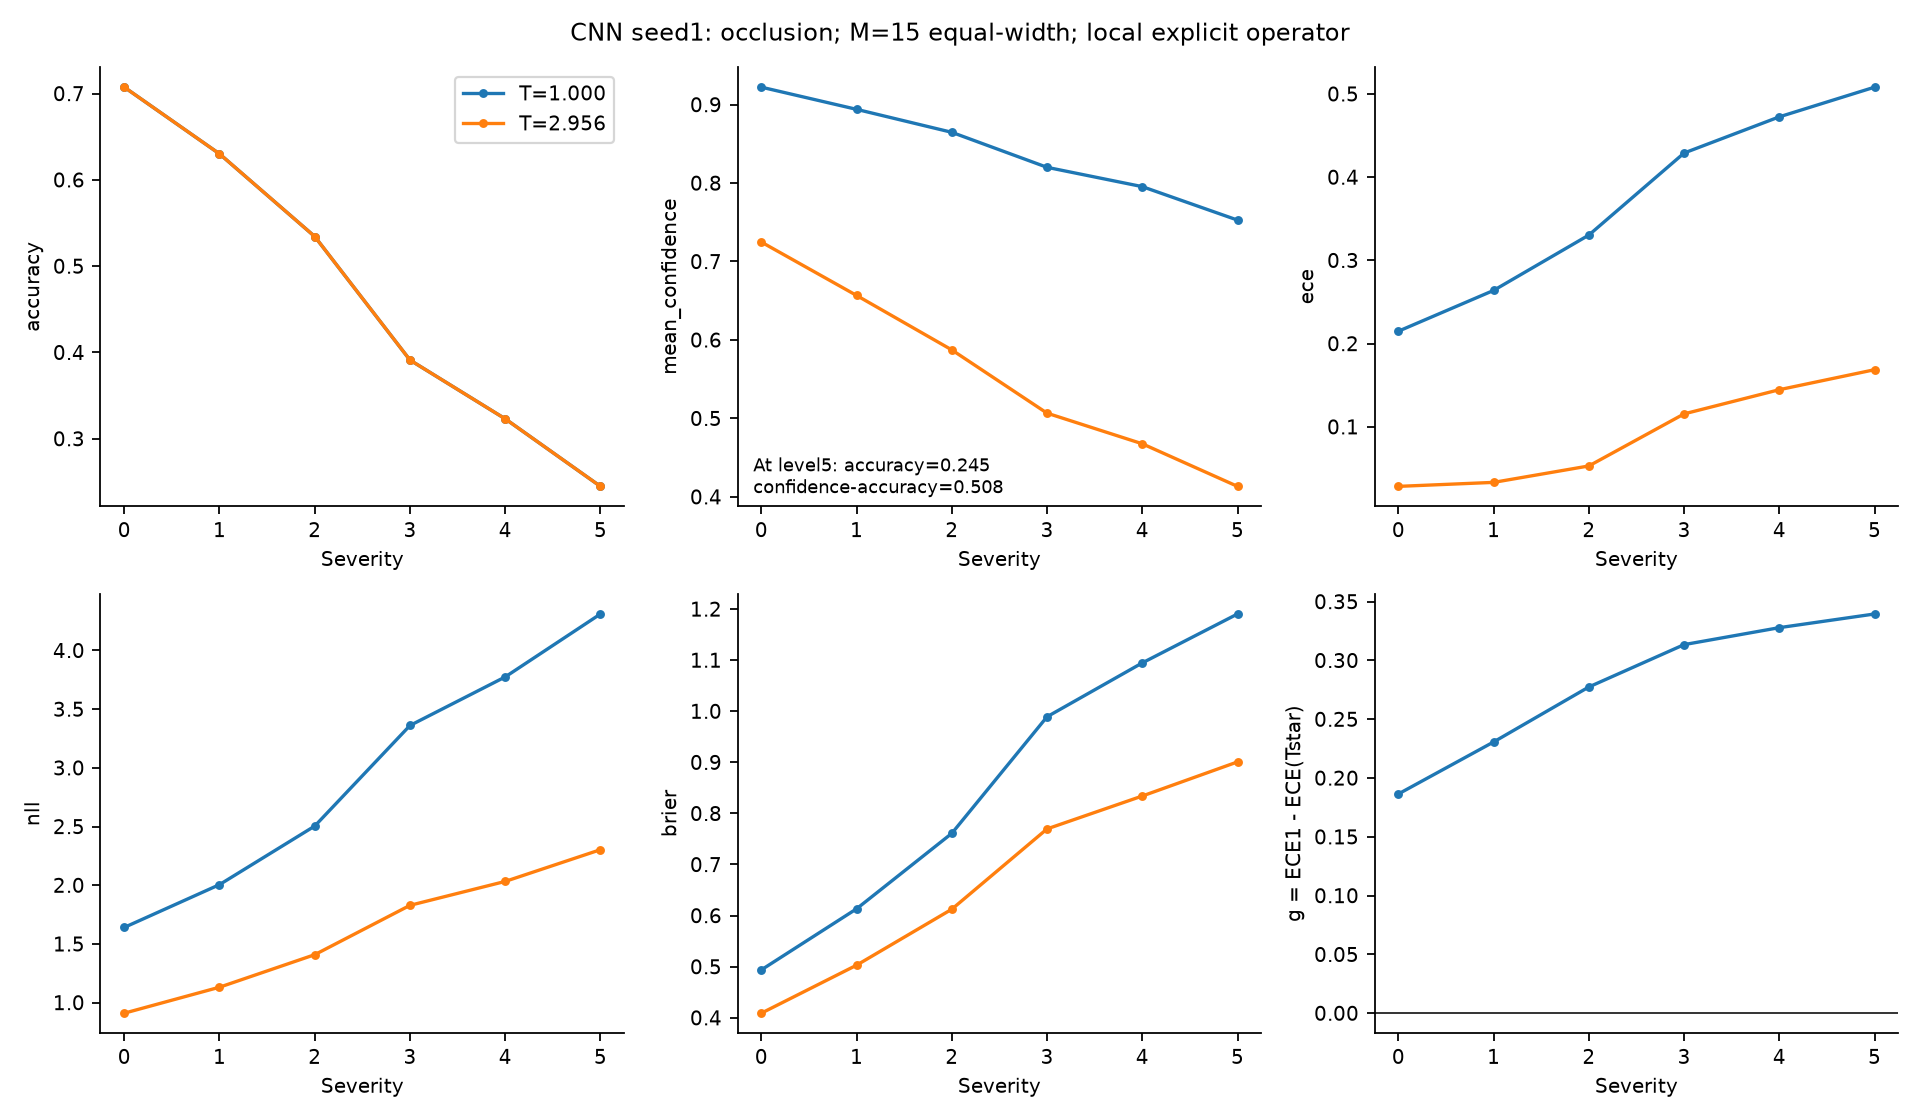
\includegraphics[width=\linewidth,height=.34\textheight,keepaspectratio]{figures/occlusion.png}
\caption{E2: Закрытие, CNN seed 1; ECE 15 equal-width, T=1 и T*=2.956378.}\label{fig:occlusion}
\end{figure}

При occlusion5 accuracy падает с 0.7074 до 0.2447, тогда как исходная confidence --- с 0.922246 до 0.752771. Модель становится гораздо менее правильной, оставаясь уверенной. Температура смягчает overconfidence, но не восстанавливает классы.

До основного сравнения ожидалось $\Delta_s=g_A(s)-g_B(s)>0$, где $g=ECE_1-ECE_{T^*}$, A --- clean, B --- occlusion5. Единственный фактор пары --- входное условие; для каждого seed одна модель и T*, подобранная на его чистой val. Три исходных checkpoint задают вариативность обучения, а не случайное разбиение test.
\begin{table}[H]\centering\footnotesize
\setlength{\tabcolsep}{4pt}
\caption{Основное сравнение E2: выигрыш температуры на clean минус occlusion5.}\label{tab:pairs}
\begin{tabular}{rrrrrl}
\toprule
Seed & $T^*$ & $g_A$ & $g_B$ & $\Delta_s$ & Ист. clean/shift \\
\midrule
1 & 2.956378 & 0.186429 & 0.339474 & -0.153045 & R05/R07 \\
2 & 3.103821 & 0.203712 & 0.362654 & -0.158942 & R08/R09 \\
3 & 3.114989 & 0.189247 & 0.363411 & -0.174164 & R10/R11 \\
\bottomrule
\end{tabular}
\end{table}


\begin{figure}[H]\centering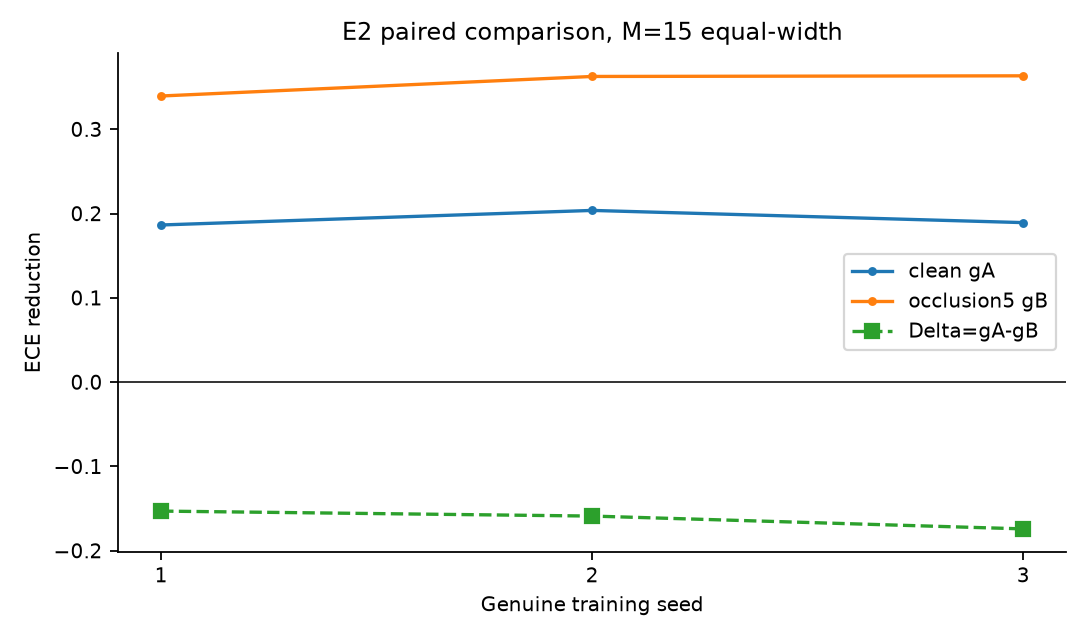
\includegraphics[width=\linewidth,height=.30\textheight,keepaspectratio]{figures/paired.png}
\caption{Три парные разности E2; положительный знак ожидался до измерения.}\label{fig:paired}
\end{figure}

Все разности отрицательны, среднее $-0.162050322$, выборочное SD 0.010897215; модуль среднего превышает $2s_\Delta=0.021794431$. Установлен обратный вывод: в этих условиях абсолютный выигрыш температуры больше на сильном искажении. Предположение о порядке выигрышей опровергнуто. Причина согласуется с намного большей исходной избыточной уверенностью на искажении. При этом итоговая ECE после T* на occlusion5 0.168598 хуже clean 0.028418, так что больший выигрыш не означает лучшую конечную калибровку.

На исследованной сетке ни одного $g\le0$ не найдено. Граница отсутствия пользы температуры лежит вне измеренных условий, если она существует. Для известного сдвига отдельно подобрана $T_5=6.108734$ на occlusion5 val.
\begin{table}[H]\centering\footnotesize
\setlength{\tabcolsep}{4pt}
\caption{Температура, подобранная на corrupted val, и её перенос на два test-условия.}\label{tab:t5}
\begin{tabular}{lrrrrrrr}
\toprule
Test & $T$ & Accuracy & Conf. & ECE & NLL & Brier & Пусто \\
\midrule
clean & 1.00000 & 0.70740 & 0.92225 & 0.21485 & 1.64031 & 0.49371 & 3 \\
clean & 2.95638 & 0.70740 & 0.72477 & 0.02842 & 0.90976 & 0.40894 & 2 \\
clean & 6.10873 & 0.70740 & 0.44196 & 0.26552 & 1.16225 & 0.49697 & 1 \\
shift5 & 1.00000 & 0.24470 & 0.75277 & 0.50807 & 4.31040 & 1.19033 & 2 \\
shift5 & 2.95638 & 0.24470 & 0.41329 & 0.16860 & 2.30249 & 0.90077 & 2 \\
shift5 & 6.10873 & 0.24470 & 0.23413 & 0.02918 & 2.14317 & 0.85721 & 5 \\
\bottomrule
\end{tabular}
\end{table}



\section{E3. Состязательные возмущения}
Атаки максимизируют CE исходной модели T=1 в eval. FGSM делает $x_{adv}=\Pi_{[0,1]}[x+\epsilon\operatorname{sign}\nabla_xL]$. PGD начинает в случайной точке допустимого шара, делает K шагов $\alpha=2.5\epsilon/K$ и после каждого проецирует на пересечение $[x-\epsilon,x+\epsilon]$ и [0,1]. При R стартах выбирается худший вариант для каждого изображения. Все ограничения заданы в исходных пикселях, параметры модели фиксированы.
\begin{table}[H]\centering\footnotesize
\setlength{\tabcolsep}{4pt}
\caption{E3: T=1, один и тот же полный test, 10 000 изображений.}\label{tab:attacks}
\begin{tabular}{lll lrrrl}
\toprule
Модель & Атака & $255\epsilon$ & K/R & Acc. & Conf. & ECE & Ист. \\
\midrule
cnn 1 & FGSM & 0 & 1/1 & 0.70740 & 0.92225 & 0.21485 & R12 \\
cnn 1 & FGSM & 1 & 1/1 & 0.47210 & 0.91979 & 0.44769 & R13 \\
cnn 1 & FGSM & 2 & 1/1 & 0.29880 & 0.92462 & 0.62592 & R14 \\
cnn 1 & FGSM & 4 & 1/1 & 0.12870 & 0.93452 & 0.80597 & R15 \\
cnn 1 & FGSM & 8 & 1/1 & 0.03440 & 0.93806 & 0.90375 & R16 \\
cnn 1 & PGD & 2.0 & 10/1 & 0.24580 & 0.95869 & 0.71303 & R17 \\
cnn 1 & PGD & 2.0 & 20/2 & 0.24310 & 0.96018 & 0.71736 & R18 \\
cnn 1 & random & 2.0 & / & 0.70570 & 0.92182 & 0.21612 & R19 \\
vit 1 & FGSM & 0 & 1/1 & 0.45020 & 0.91751 & 0.46731 & R20 \\
vit 1 & FGSM & 1 & 1/1 & 0.21000 & 0.94867 & 0.73867 & R21 \\
vit 1 & FGSM & 2 & 1/1 & 0.10310 & 0.96118 & 0.85808 & R22 \\
vit 1 & FGSM & 4 & 1/1 & 0.04030 & 0.96663 & 0.92633 & R23 \\
vit 1 & FGSM & 8 & 1/1 & 0.01740 & 0.95602 & 0.93862 & R24 \\
vit 1 & PGD & 2.0 & 10/1 & 0.07600 & 0.98578 & 0.90978 & R25 \\
vit 1 & PGD & 2.0 & 20/2 & 0.07540 & 0.98618 & 0.91109 & R26 \\
vit 1 & random & 2.0 & / & 0.44890 & 0.91775 & 0.46885 & R27 \\
\bottomrule
\end{tabular}
\end{table}


\begin{figure}[H]\centering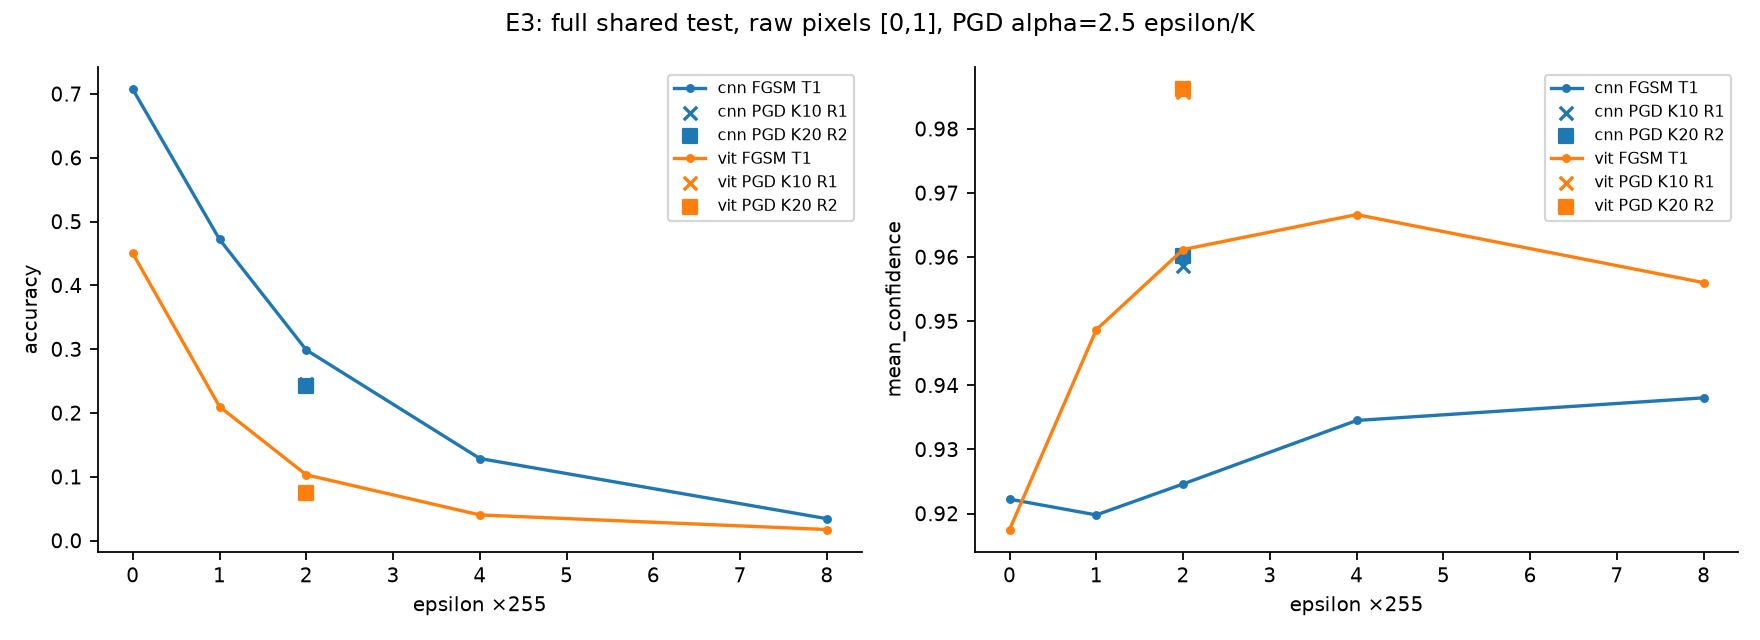
\includegraphics[width=\linewidth,height=.37\textheight,keepaspectratio]{figures/attackfig.png}
\caption{FGSM eps=0,1,2,4,8 /255 и PGD eps=2/255, K10 R1 и K20 R2, alpha=2.5 eps/K.}\label{fig:attackfig}
\end{figure}

PGD10 даёт accuracy 0.2458/0.0760 для CNN/ViT против FGSM 0.2988/0.1031 при том же $\epsilon=2/255$. Усиление до K20,R2 снижает их до 0.2431/0.0754: десять шагов ещё не дали окончательной оценки. Во всех реальных примерах и шагах PGD выполнены Linf и диапазон; при нулевом epsilon результат совпадает с чистым test.
\begin{figure}[H]\centering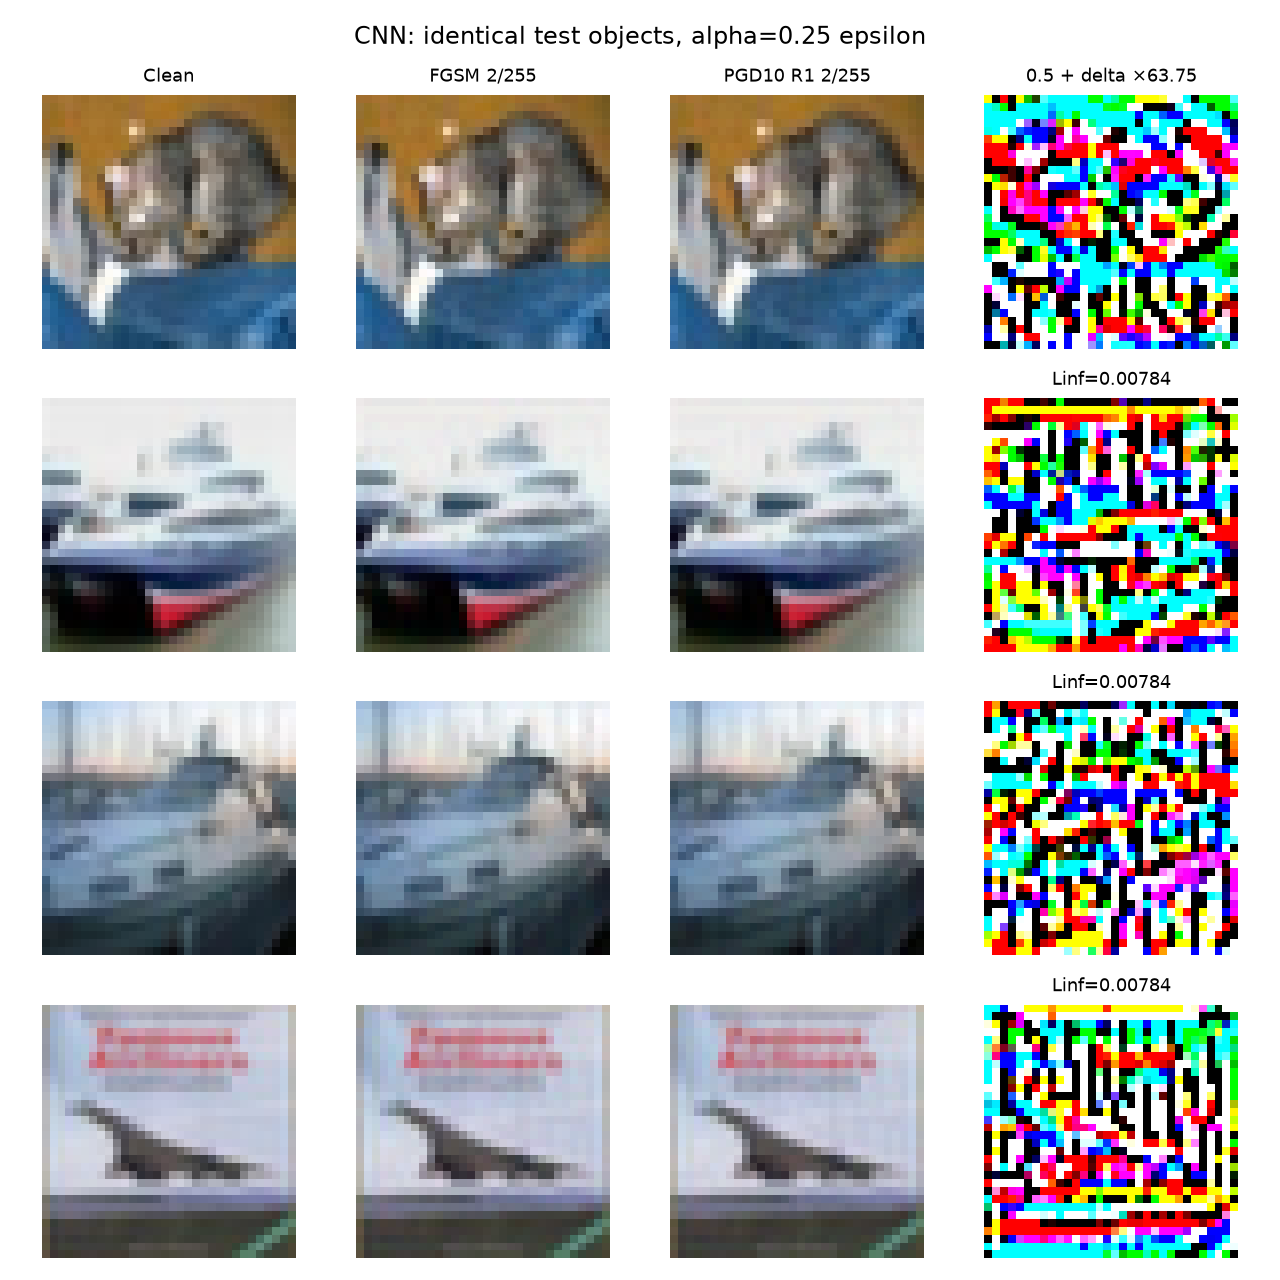
\includegraphics[width=\linewidth,height=.42\textheight,keepaspectratio]{figures/examplecnn.png}
\caption{CNN: исходные и атакованные изображения, усиленное возмущение и его Linf-норма.}\label{fig:examplecnn}
\end{figure}

\begin{figure}[H]\centering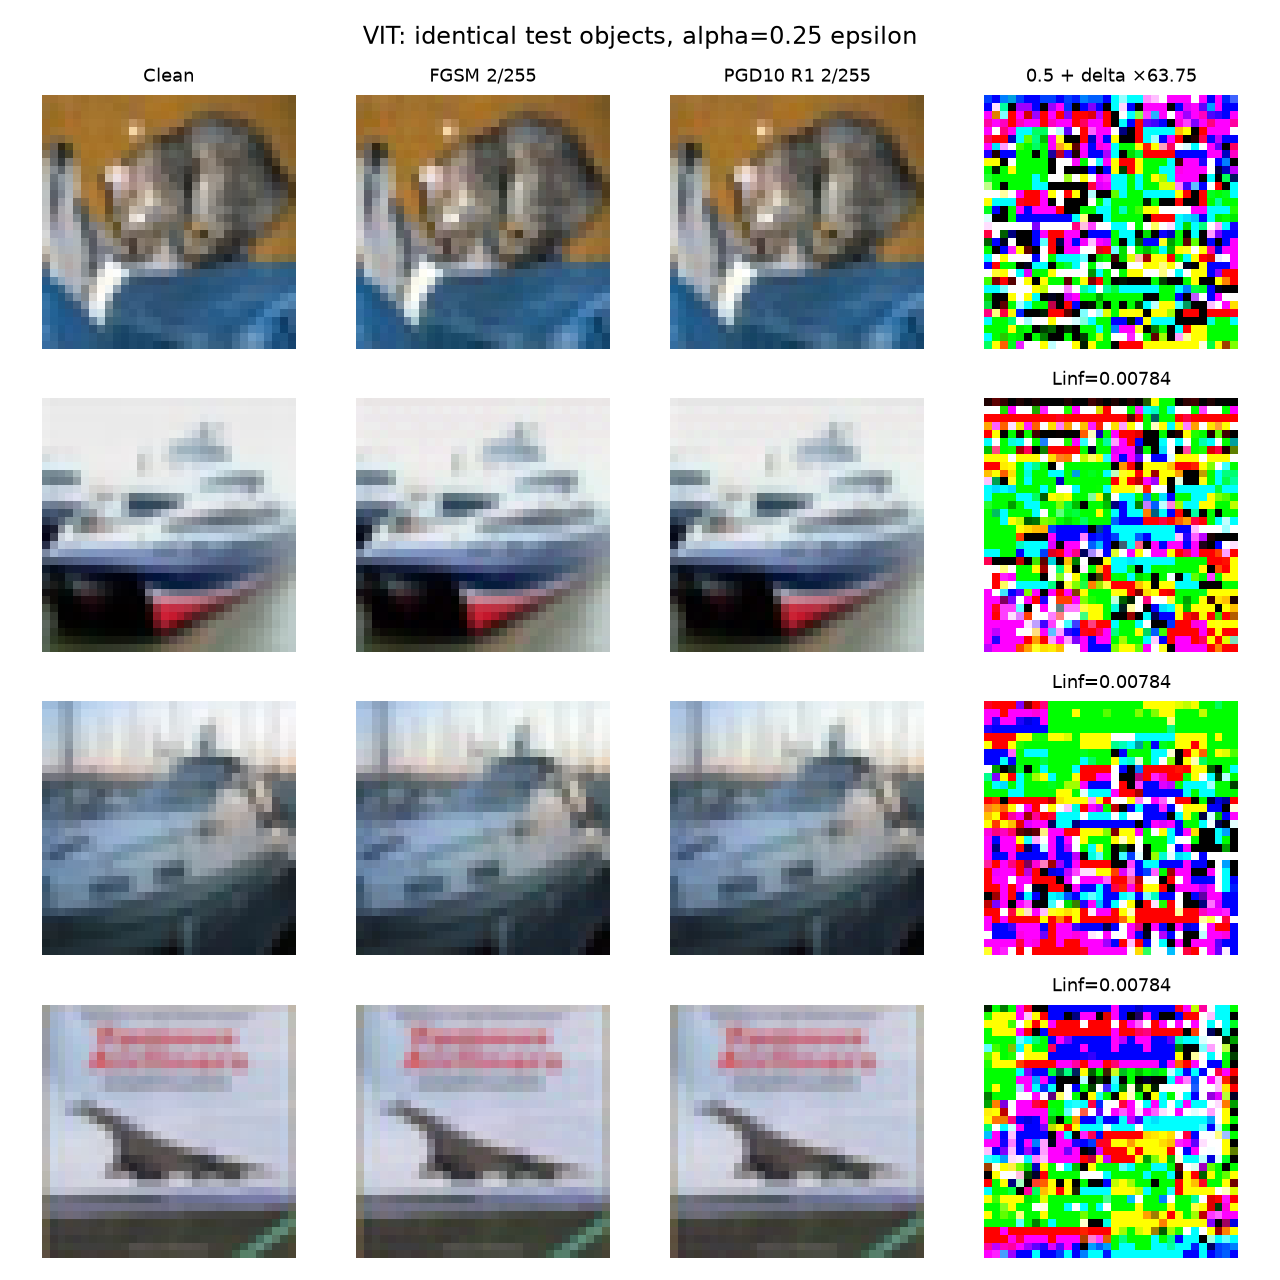
\includegraphics[width=\linewidth,height=.42\textheight,keepaspectratio]{figures/examplevit.png}
\caption{ViT: соответствующие примеры на тех же test ID.}\label{fig:examplevit}
\end{figure}

Точность под конкретной атакой --- верхняя оценка устойчивости к наихудшему допустимому возмущению. Она не является сертификатом против любых атак. Высокая confidence после атаки может сопровождать почти всегда неверный класс.

\section{Профиль надёжности: отказ и OOD}
Модель отвечает при $U\le\tau$. Coverage --- доля принятых, risk --- доля ошибок среди них. При нулевом coverage риск не определён. AURC --- средний накопленный риск при сортировке U по возрастанию. Вместе с AURC показан избыток над oracle, ставящим ошибки в конец; это учитывает различную исходную accuracy моделей.

В OOD-задаче положительный класс --- SVHN. AUROC оценивает вероятность большего U у OOD с половинным весом ties; FPR95 --- доля ID, отклонённых при обнаружении не менее 95\% OOD. AUPR зависит от доли OOD: здесь $26032/(26032+10000)=0.72247$. Смысловые метки SVHN не используются.
\begin{table}[H]\centering\scriptsize
\setlength{\tabcolsep}{4pt}
\caption{Selective и semantic OOD: меньше AURC и FPR95, больше AUROC/AUPR лучше.}\label{tab:ood}
\begin{tabular}{ll lrrrrr}
\toprule
Модель & $T$ & Мера & AURC & Избыток & AUROC & AUPR & FPR95 \\
\midrule
cnn 1 & 1.000 & msp & 0.1159 & 0.0682 & 0.6741 & 0.8042 & 0.7037 \\
cnn 1 & 1.000 & entropy & 0.1154 & 0.0677 & 0.6730 & 0.7999 & 0.7034 \\
cnn 1 & 1.000 & margin & 0.1164 & 0.0687 & 0.6744 & 0.8067 & 0.7042 \\
cnn 1 & 2.956 & msp & 0.1150 & 0.0672 & 0.6673 & 0.7935 & 0.7057 \\
cnn 1 & 2.956 & entropy & 0.1164 & 0.0687 & 0.6557 & 0.7777 & 0.7092 \\
cnn 1 & 2.956 & margin & 0.1155 & 0.0678 & 0.6724 & 0.8047 & 0.7047 \\
vit 1 & 1.000 & msp & 0.3931 & 0.2025 & 0.5789 & 0.7600 & 0.8640 \\
vit 1 & 1.000 & entropy & 0.3919 & 0.2014 & 0.5803 & 0.7619 & 0.8632 \\
vit 1 & 1.000 & margin & 0.3947 & 0.2042 & 0.5779 & 0.7591 & 0.8658 \\
vit 1 & 4.273 & msp & 0.3850 & 0.1945 & 0.5920 & 0.7680 & 0.8530 \\
vit 1 & 4.273 & entropy & 0.3825 & 0.1920 & 0.6025 & 0.7729 & 0.8480 \\
vit 1 & 4.273 & margin & 0.3901 & 0.1995 & 0.5834 & 0.7616 & 0.8572 \\
cnn 2 & 1.000 & msp & 0.1251 & 0.0705 & 0.6601 & 0.7981 & 0.7306 \\
cnn 2 & 1.000 & entropy & 0.1245 & 0.0700 & 0.6600 & 0.7957 & 0.7299 \\
cnn 2 & 1.000 & margin & 0.1257 & 0.0711 & 0.6597 & 0.7993 & 0.7325 \\
cnn 2 & 3.104 & msp & 0.1227 & 0.0681 & 0.6595 & 0.7938 & 0.7286 \\
cnn 2 & 3.104 & entropy & 0.1236 & 0.0690 & 0.6548 & 0.7872 & 0.7308 \\
cnn 2 & 3.104 & margin & 0.1240 & 0.0695 & 0.6601 & 0.7991 & 0.7279 \\
cnn 3 & 1.000 & msp & 0.1111 & 0.0650 & 0.6396 & 0.7889 & 0.7623 \\
cnn 3 & 1.000 & entropy & 0.1107 & 0.0647 & 0.6396 & 0.7892 & 0.7622 \\
cnn 3 & 1.000 & margin & 0.1115 & 0.0655 & 0.6391 & 0.7873 & 0.7619 \\
cnn 3 & 3.115 & msp & 0.1100 & 0.0640 & 0.6378 & 0.7864 & 0.7570 \\
cnn 3 & 3.115 & entropy & 0.1117 & 0.0656 & 0.6320 & 0.7820 & 0.7577 \\
cnn 3 & 3.115 & margin & 0.1105 & 0.0645 & 0.6392 & 0.7867 & 0.7580 \\
\bottomrule
\end{tabular}
\end{table}


\begin{figure}[H]\centering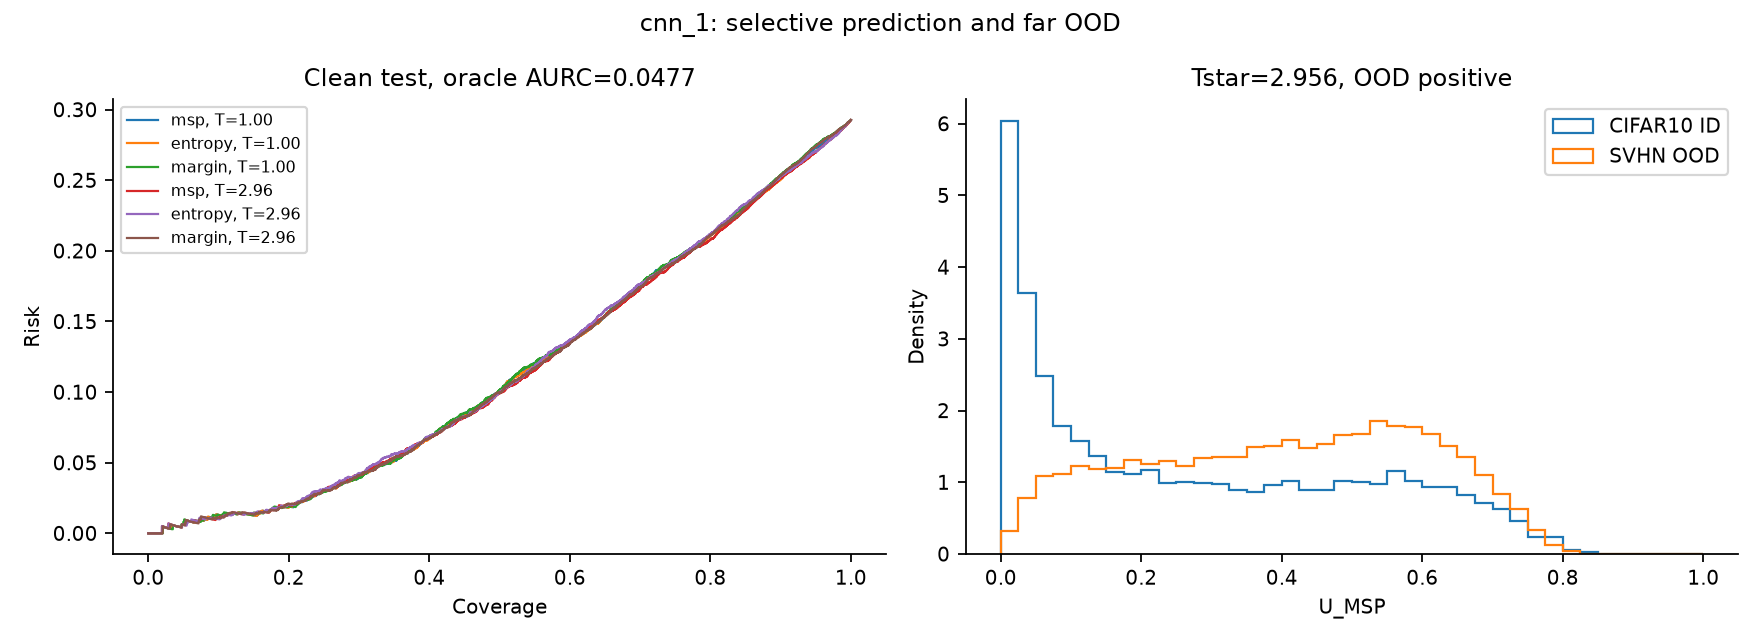
\includegraphics[width=\linewidth,height=.37\textheight,keepaspectratio]{figures/riskcnn.png}
\caption{CNN seed 1: risk--coverage и OOD при T=1 / T*=2.956378.}\label{fig:riskcnn}
\end{figure}

\begin{figure}[H]\centering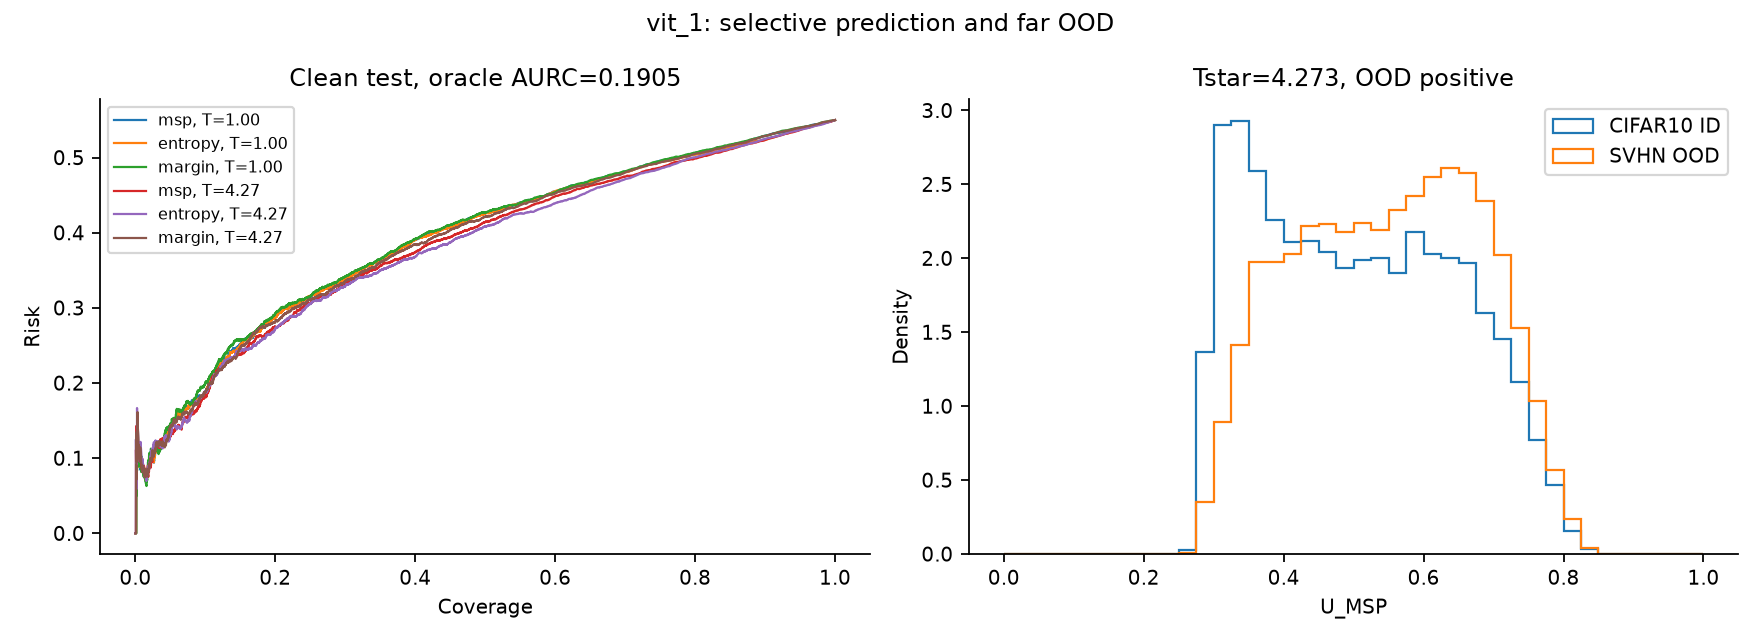
\includegraphics[width=\linewidth,height=.37\textheight,keepaspectratio]{figures/riskvit.png}
\caption{ViT seed 1: risk--coverage и OOD при T=1 / T*=4.273313.}\label{fig:riskvit}
\end{figure}

\begin{figure}[H]\centering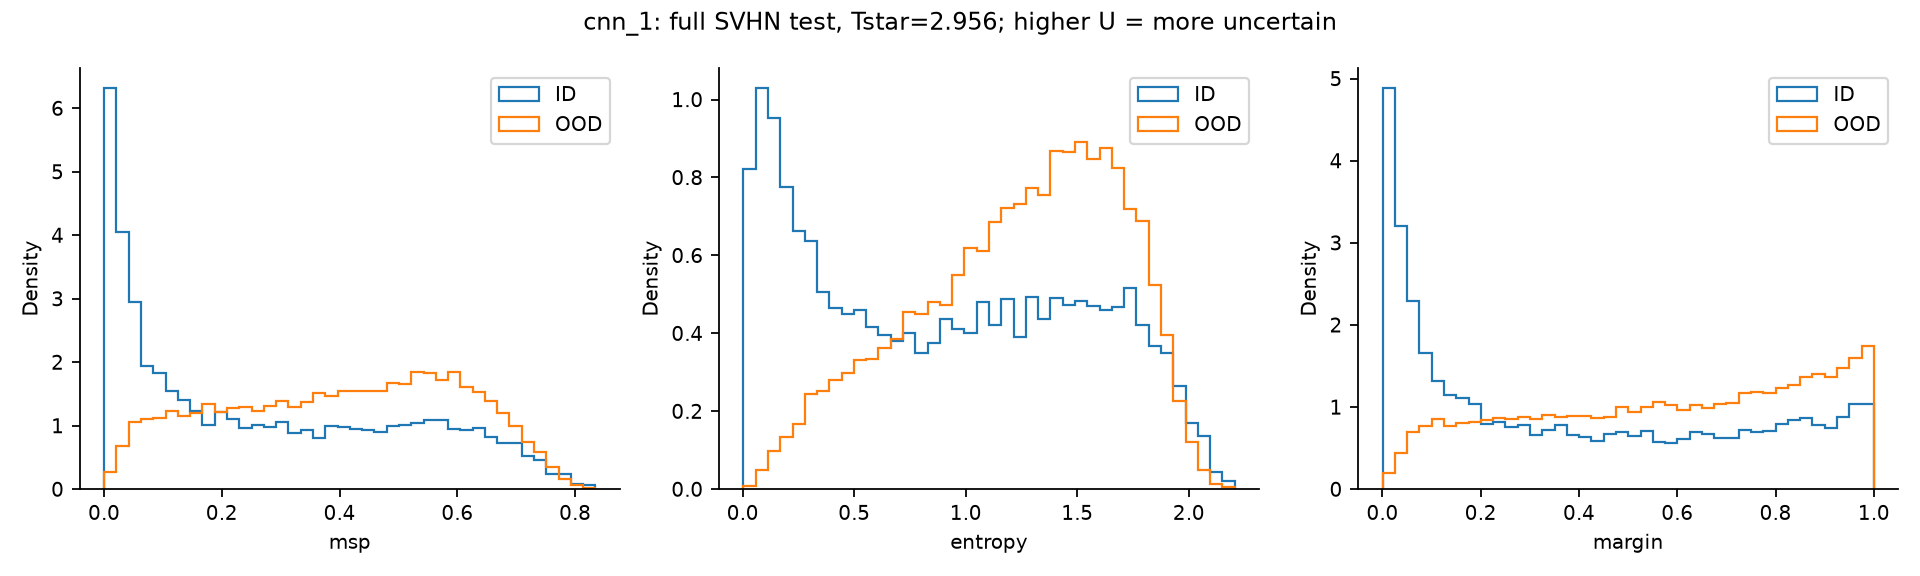
\includegraphics[width=\linewidth,height=.36\textheight,keepaspectratio]{figures/oodcnn.png}
\caption{Распределения трёх мер неопределённости CNN на CIFAR-10 и SVHN.}\label{fig:oodcnn}
\end{figure}

\begin{figure}[H]\centering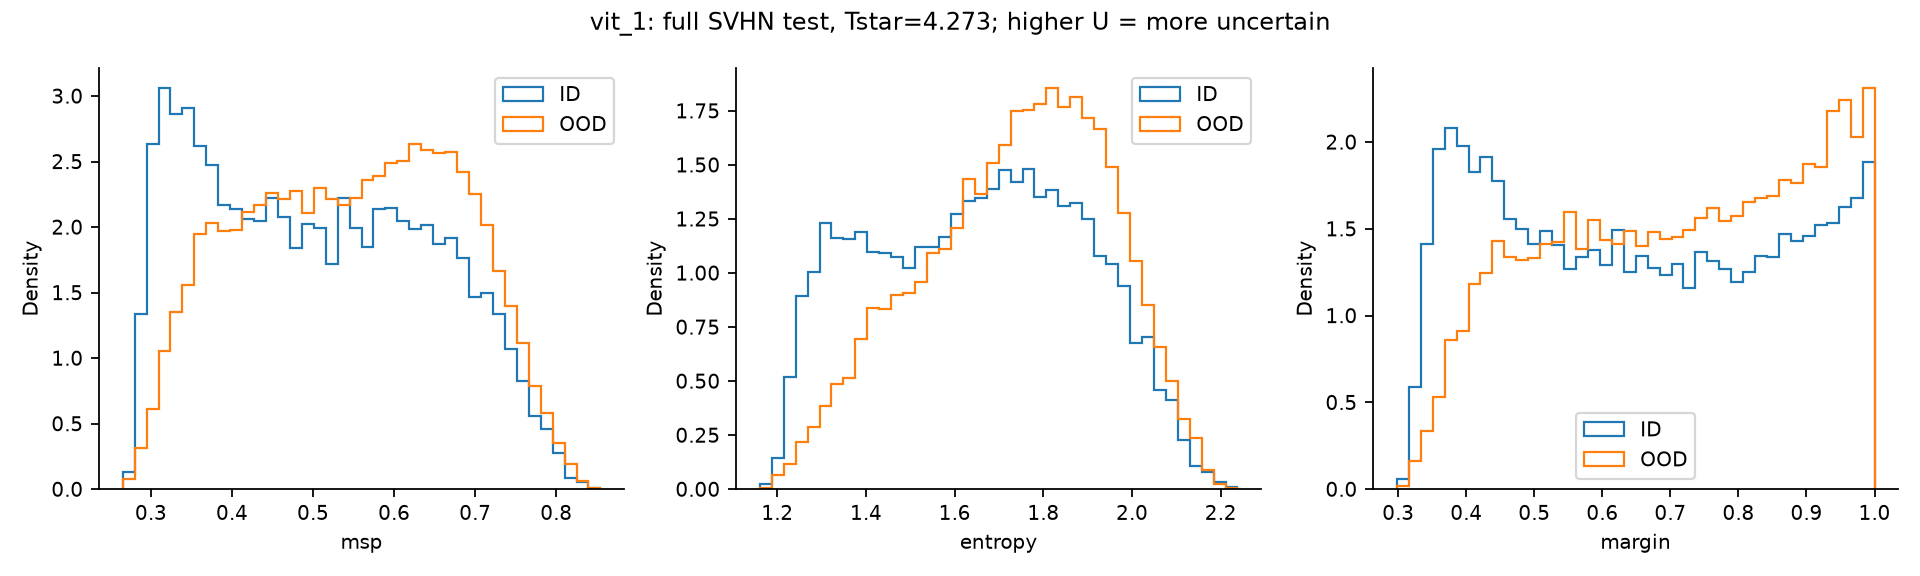
\includegraphics[width=\linewidth,height=.36\textheight,keepaspectratio]{figures/oodvit.png}
\caption{Распределения трёх мер неопределённости ViT на CIFAR-10 и SVHN.}\label{fig:oodvit}
\end{figure}

Для CNN seed 1 MSP-AURC 0.115934 при oracle 0.047742, после T* 0.114975; AUROC 0.674099 уменьшается до 0.667306. Для ViT AURC 0.393064 уменьшается до 0.385041, AUROC 0.578933 растёт до 0.592006. Хорошая калибровка на clean не обеспечила сильного разделения semantic OOD.

На SVHN accuracy, ECE, NLL и Brier не определены: в десяти классах CIFAR-10 нет правильного класса цифры. В профиле также не заявлены conformal coverage, near-OOD и ансамбль. Оценки относятся к измеренным искажениям, epsilon и далёкому OOD; будущий неизвестный сдвиг не покрыт.

\section{Ответы на контрфактические вопросы}
\subsection*{Вопрос 1. ECE против NLL и Brier}
У CNN изменения после T*: ECE $-0.186429$, NLL $-0.730550$, Brier $-0.084769$; у ViT $-0.400536,-2.390522,-0.278635$. Все улучшились, измеренного контрпримера нет. Теоретически снижение ECE не гарантирует снижения NLL/Brier, поскольку они учитывают разные аспекты вероятностей. Val NLL не растёт из-за целевой минимизации с включённым T=1; на test такой гарантии нет.
\subsection*{Вопрос 2. T5 на clean и shift}
Относительно T* температура T5 уменьшает occlusion5 ECE с 0.168598 до 0.029181, NLL с 2.302492 до 2.143172, Brier с 0.900775 до 0.857212. На clean ECE растёт с 0.028418 до 0.265515, NLL с 0.909765 до 1.162255, Brier с 0.408943 до 0.496966. T5 соответствует известному сдвигу, но не является универсальным калибратором. Для будущего неизвестного сдвига такой val заранее нет.
\subsection*{Вопрос 3. Случайный знак при той же норме}
При $\epsilon=2/255$ случайный знак даёт accuracy CNN 0.7057 и ViT 0.4489, FGSM 0.2988/0.1031, PGD10 0.2458/0.0760. Предсказанный порядок random $>$ FGSM $\ge$ PGD подтвердился на общих ID. Случайное направление не согласовано с градиентом CE, тогда как FGSM максимизирует линейное приближение; одна норма не определяет вред возмущения.
\subsection*{Вопрос 4. Температура и уверенные ошибки}
На FGSM $2/255$ CNN confidence меняется 0.924621 $\to$ 0.717081, ECE 0.625821 $\to$ 0.418460; ViT 0.961179 $\to$ 0.572030, ECE 0.858079 $\to$ 0.468930. Изменённых предсказаний и исправленных ошибочных классов нет. Температура корректирует вероятности, а не классификационное решение.
\subsection*{Вопрос 5. Ранжирование объектов}
MSP-AURC и AUROC до/после приведены в профиле. Позиции в сортировке ID изменились у 9973 объектов CNN и 9981 ViT, классы --- у нуля. Температура сохраняет порядок логитов внутри изображения, но не обязана сохранять порядок максимальных вероятностей между изображениями. Инвариантность AUROC относится к строго возрастающему преобразованию уже готового скалярного U, а softmax(z/T) не является одним таким преобразованием MSP для всех векторов z.

\noindent\textbf{Заключение.} Температура улучшила калибровку, но не исправила классы и не гарантировала надёжность при сдвиге.
\clearpage
\renewcommand{\refname}{Список использованных источников}
\begin{thebibliography}{9}
\addcontentsline{toc}{section}{Список использованных источников}
\bibitem{teacher} Лабораторная работа 8. Когда предсказанию сети можно доверять. Надёжность, калибровка и неопределённость. Курс «Нейронные сети». Методические указания, 2026.
\end{thebibliography}
\clearpage
\section*{Приложение. Идентификация запусков}
\addcontentsline{toc}{section}{Приложение. Идентификация запусков}
\begingroup\small\setstretch{1.05}
\begin{longtable}{@{}l>{\raggedright\arraybackslash}p{3.5cm}p{10.8cm}@{}}
\caption{Полные RUN\_ID источников результатов.}\\
\toprule Код & Условие & RUN\_ID \\ \midrule \endhead
\hypertarget{R01}{R01} & Lab2 cnn 1 & {\fontsize{8.8}{11}\selectfont\texttt{8705d516f9c58ae4458c-2297f86c299c4b998e5a33258a6b8326}} \\
\hypertarget{R02}{R02} & Lab2 cnn 2 & {\fontsize{8.8}{11}\selectfont\texttt{f1a84ec3e8723294d4a2-14cad9141a774b6daee3100c969640f6}} \\
\hypertarget{R03}{R03} & Lab2 cnn 3 & {\fontsize{8.8}{11}\selectfont\texttt{69ac6bd9ed94ae61d1aa-873bbd5089054e138a586cd2a337e139}} \\
\hypertarget{R04}{R04} & Lab2 vit 1 & {\fontsize{8.8}{11}\selectfont\texttt{76a6bee7ce9731bfa4fa-8edbe989a96e427c82f75e87ddd2c0ab}} \\
\hypertarget{R05}{R05} & E1 cnn & {\fontsize{8.8}{11}\selectfont\texttt{73968c7a84a5394c6aa0-5b8b87df36624d71a8c08781804ed7fd}} \\
\hypertarget{R06}{R06} & E1 vit & {\fontsize{8.8}{11}\selectfont\texttt{0799d8eab079cab5e620-ec0903e00a2f4df899b1f979e3032c7c}} \\
\hypertarget{R07}{R07} & E2 occ5 s1 & {\fontsize{8.8}{11}\selectfont\texttt{d916efcb86dbc37ed0fd-5ea6c8d7ae3a4713abdc9196f866be8f}} \\
\hypertarget{R08}{R08} & E2 clean s2 & {\fontsize{8.8}{11}\selectfont\texttt{adf7875f58dc5a33abcb-9beff1f907e6459d9241c8da09dcbf6d}} \\
\hypertarget{R09}{R09} & E2 occ5 s2 & {\fontsize{8.8}{11}\selectfont\texttt{1b9e2c8adc87da51f43e-21c97ce47ce14c5094c6d8f322577b71}} \\
\hypertarget{R10}{R10} & E2 clean s3 & {\fontsize{8.8}{11}\selectfont\texttt{fb2bf5669b606f7353b3-fb200b8facea453892a7cb99672a9126}} \\
\hypertarget{R11}{R11} & E2 occ5 s3 & {\fontsize{8.8}{11}\selectfont\texttt{9fbe4b23ef2186c639a8-621b2bf393314d84992ba240404c4b4e}} \\
\hypertarget{R12}{R12} & cnn 1 FGSM eps0 K1 & {\fontsize{8.8}{11}\selectfont\texttt{f669bc74fac0f59ecb07-92578798ac0a4ac881373db791f892a9}} \\
\hypertarget{R13}{R13} & cnn 1 FGSM eps1 K1 & {\fontsize{8.8}{11}\selectfont\texttt{269235b4e42469f1f427-31afe187d8874ccd90810cd729cb9751}} \\
\hypertarget{R14}{R14} & cnn 1 FGSM eps2 K1 & {\fontsize{8.8}{11}\selectfont\texttt{1a44bb9104623fa07cb4-60472984ecd94626b9d910b76e11e7c3}} \\
\hypertarget{R15}{R15} & cnn 1 FGSM eps4 K1 & {\fontsize{8.8}{11}\selectfont\texttt{9e73f0a9a788cd0a7e15-633c44687fba46c7b47e051459944848}} \\
\hypertarget{R16}{R16} & cnn 1 FGSM eps8 K1 & {\fontsize{8.8}{11}\selectfont\texttt{e2b28e527a75a35a8c24-4ddb2e6f24c54581951d73310baa4fbd}} \\
\hypertarget{R17}{R17} & cnn 1 PGD eps2.0 K10 & {\fontsize{8.8}{11}\selectfont\texttt{00aed6b3019eda8bd2b0-e1833f1367e4430f8aeccd94a49d11b6}} \\
\hypertarget{R18}{R18} & cnn 1 PGD eps2.0 K20 & {\fontsize{8.8}{11}\selectfont\texttt{669f74441c1d0bdf9cf6-ef275b8799014ee79fb03a5693b2d6ee}} \\
\hypertarget{R19}{R19} & cnn 1 random eps2.0 K & {\fontsize{8.8}{11}\selectfont\texttt{07fec26d48c701023bbd-28ec2dc11eff416185d2bb75ca985d2f}} \\
\hypertarget{R20}{R20} & vit 1 FGSM eps0 K1 & {\fontsize{8.8}{11}\selectfont\texttt{a05b46698998adbde31d-f3ad6d2937eb4c93b6b015c90911a9e0}} \\
\hypertarget{R21}{R21} & vit 1 FGSM eps1 K1 & {\fontsize{8.8}{11}\selectfont\texttt{22db9ba6ab867bcc1d57-e727981c4ca647488299d2fa01151396}} \\
\hypertarget{R22}{R22} & vit 1 FGSM eps2 K1 & {\fontsize{8.8}{11}\selectfont\texttt{be749c9af8d7ccb534e2-69374eeafcc54854810477dd4e5d9500}} \\
\hypertarget{R23}{R23} & vit 1 FGSM eps4 K1 & {\fontsize{8.8}{11}\selectfont\texttt{82a6087687cc2c8c5c9b-19454af7b1184b9299a761b6bea4cf27}} \\
\hypertarget{R24}{R24} & vit 1 FGSM eps8 K1 & {\fontsize{8.8}{11}\selectfont\texttt{8d1e5819f7bc0d28b6dd-c705a88f9353488ab16a0427fcb193ef}} \\
\hypertarget{R25}{R25} & vit 1 PGD eps2.0 K10 & {\fontsize{8.8}{11}\selectfont\texttt{79a1b4800fce5956a2d9-2d085f1bce3b439aa37201e020dabd75}} \\
\hypertarget{R26}{R26} & vit 1 PGD eps2.0 K20 & {\fontsize{8.8}{11}\selectfont\texttt{f43e239aca6b8f9a3c27-6d81a2d31c5a46c59dd4c858023ddcfd}} \\
\hypertarget{R27}{R27} & vit 1 random eps2.0 K & {\fontsize{8.8}{11}\selectfont\texttt{4ed189b2245186f3b436-7011dd2f77284357931c0e901a28d9d2}} \\
\hypertarget{R28}{R28} & selective OOD cnn 1 & {\fontsize{8.8}{11}\selectfont\texttt{c4bd07267e884795ad42-9f79f9e6c4534bf9ae92ce4d5fbd849f}} \\
\hypertarget{R29}{R29} & selective OOD vit 1 & {\fontsize{8.8}{11}\selectfont\texttt{28c6a867fdd60b50e742-b8ff8463a4ac44f38517e4b96fe64ebe}} \\
\hypertarget{R30}{R30} & selective OOD cnn 2 & {\fontsize{8.8}{11}\selectfont\texttt{ee51a112fbd8ca02ceac-0fbadfbec7b946c6b6e26b3bedc5b2a1}} \\
\hypertarget{R31}{R31} & selective OOD cnn 3 & {\fontsize{8.8}{11}\selectfont\texttt{62769d38becb70261a95-0f87c25adf8344b599bf1396638e8f47}} \\
\bottomrule\end{longtable}\endgroup
